\documentclass[twoside]{book}

% Packages required by doxygen
\usepackage{calc}
\usepackage{doxygen}
\usepackage{graphicx}
\usepackage[utf8]{inputenc}
\usepackage{makeidx}
\usepackage{multicol}
\usepackage{multirow}
\usepackage{textcomp}
\usepackage[table]{xcolor}

% Font selection
\usepackage[T1]{fontenc}
\usepackage{mathptmx}
\usepackage[scaled=.90]{helvet}
\usepackage{courier}
\usepackage{amssymb}
\usepackage{sectsty}
\renewcommand{\familydefault}{\sfdefault}
\allsectionsfont{%
  \fontseries{bc}\selectfont%
  \color{darkgray}%
}
\renewcommand{\DoxyLabelFont}{%
  \fontseries{bc}\selectfont%
  \color{darkgray}%
}

% Page & text layout
\usepackage{geometry}
\geometry{%
  a4paper,%
  top=2.5cm,%
  bottom=2.5cm,%
  left=2.5cm,%
  right=2.5cm%
}
\tolerance=750
\hfuzz=15pt
\hbadness=750
\setlength{\emergencystretch}{15pt}
\setlength{\parindent}{0cm}
\setlength{\parskip}{0.2cm}
\makeatletter
\renewcommand{\paragraph}{%
  \@startsection{paragraph}{4}{0ex}{-1.0ex}{1.0ex}{%
    \normalfont\normalsize\bfseries\SS@parafont%
  }%
}
\renewcommand{\subparagraph}{%
  \@startsection{subparagraph}{5}{0ex}{-1.0ex}{1.0ex}{%
    \normalfont\normalsize\bfseries\SS@subparafont%
  }%
}
\makeatother

% Headers & footers
\usepackage{fancyhdr}
\pagestyle{fancyplain}
\fancyhead[LE]{\fancyplain{}{\bfseries\thepage}}
\fancyhead[CE]{\fancyplain{}{}}
\fancyhead[RE]{\fancyplain{}{\bfseries\leftmark}}
\fancyhead[LO]{\fancyplain{}{\bfseries\rightmark}}
\fancyhead[CO]{\fancyplain{}{}}
\fancyhead[RO]{\fancyplain{}{\bfseries\thepage}}
\fancyfoot[LE]{\fancyplain{}{}}
\fancyfoot[CE]{\fancyplain{}{}}
\fancyfoot[RE]{\fancyplain{}{\bfseries\scriptsize Generated on Tue Oct 18 2016 13\-:06\-:45 for Document\-Class\-Hierarchy by Doxygen }}
\fancyfoot[LO]{\fancyplain{}{\bfseries\scriptsize Generated on Tue Oct 18 2016 13\-:06\-:45 for Document\-Class\-Hierarchy by Doxygen }}
\fancyfoot[CO]{\fancyplain{}{}}
\fancyfoot[RO]{\fancyplain{}{}}
\renewcommand{\footrulewidth}{0.4pt}
\renewcommand{\chaptermark}[1]{%
  \markboth{#1}{}%
}
\renewcommand{\sectionmark}[1]{%
  \markright{\thesection\ #1}%
}

% Indices & bibliography
\usepackage{natbib}
\usepackage[titles]{tocloft}
\setcounter{tocdepth}{3}
\setcounter{secnumdepth}{5}
\makeindex

% Hyperlinks (required, but should be loaded last)
\usepackage{ifpdf}
\ifpdf
  \usepackage[pdftex,pagebackref=true]{hyperref}
\else
  \usepackage[ps2pdf,pagebackref=true]{hyperref}
\fi
\hypersetup{%
  colorlinks=true,%
  linkcolor=blue,%
  citecolor=blue,%
  unicode%
}

% Custom commands
\newcommand{\clearemptydoublepage}{%
  \newpage{\pagestyle{empty}\cleardoublepage}%
}


%===== C O N T E N T S =====

\begin{document}

% Titlepage & ToC
\hypersetup{pageanchor=false}
\pagenumbering{roman}
\begin{titlepage}
\vspace*{7cm}
\begin{center}%
{\Large Document\-Class\-Hierarchy }\\
\vspace*{1cm}
{\large Generated by Doxygen 1.8.6}\\
\vspace*{0.5cm}
{\small Tue Oct 18 2016 13:06:45}\\
\end{center}
\end{titlepage}
\clearemptydoublepage
\tableofcontents
\clearemptydoublepage
\pagenumbering{arabic}
\hypersetup{pageanchor=true}

%--- Begin generated contents ---
\chapter{Namespace Index}
\section{Namespace List}
Here is a list of all documented namespaces with brief descriptions\-:\begin{DoxyCompactList}
\item\contentsline{section}{\hyperlink{namespacedocs}{docs} \\*This namespace is used to collect all the document hierarchy classes and types }{\pageref{namespacedocs}}{}
\item\contentsline{section}{\hyperlink{namespaceparray}{parray} \\*It specify the dynamic array manager for a generic data T and a std\-::string specialisation }{\pageref{namespaceparray}}{}
\item\contentsline{section}{\hyperlink{namespacepatch}{patch} \\*To emulate C++11 and get to\-\_\-string translator }{\pageref{namespacepatch}}{}
\end{DoxyCompactList}

\chapter{Hierarchical Index}
\section{Class Hierarchy}
This inheritance list is sorted roughly, but not completely, alphabetically\-:\begin{DoxyCompactList}
\item \contentsline{section}{docs\-:\-:Doc\-Type}{\pageref{classdocs_1_1DocType}}{}
\item \contentsline{section}{docs\-:\-:Document}{\pageref{classdocs_1_1Document}}{}
\begin{DoxyCompactList}
\item \contentsline{section}{docs\-:\-:Spreadsheet}{\pageref{classdocs_1_1Spreadsheet}}{}
\item \contentsline{section}{docs\-:\-:Web\-Page}{\pageref{classdocs_1_1WebPage}}{}
\end{DoxyCompactList}
\item \contentsline{section}{parray\-:\-:Pointer\-Array$<$ T $>$}{\pageref{classparray_1_1PointerArray}}{}
\item \contentsline{section}{parray\-:\-:Pointer\-Array$<$ std\-:\-:string $>$}{\pageref{classparray_1_1PointerArray}}{}
\begin{DoxyCompactList}
\item \contentsline{section}{parray\-:\-:String\-Pointer\-Array}{\pageref{classparray_1_1StringPointerArray}}{}
\end{DoxyCompactList}
\end{DoxyCompactList}

\chapter{Class Index}
\section{Class List}
Here are the classes, structs, unions and interfaces with brief descriptions\-:\begin{DoxyCompactList}
\item\contentsline{section}{\hyperlink{classdocs_1_1DocType}{docs\-::\-Doc\-Type} }{\pageref{classdocs_1_1DocType}}{}
\item\contentsline{section}{\hyperlink{classdocs_1_1Document}{docs\-::\-Document} }{\pageref{classdocs_1_1Document}}{}
\item\contentsline{section}{\hyperlink{classparray_1_1PointerArray}{parray\-::\-Pointer\-Array$<$ T $>$} \\*This class describes a manager of a dynamic array of generic type T$\ast$ }{\pageref{classparray_1_1PointerArray}}{}
\item\contentsline{section}{\hyperlink{classdocs_1_1Spreadsheet}{docs\-::\-Spreadsheet} }{\pageref{classdocs_1_1Spreadsheet}}{}
\item\contentsline{section}{\hyperlink{classparray_1_1StringPointerArray}{parray\-::\-String\-Pointer\-Array} }{\pageref{classparray_1_1StringPointerArray}}{}
\item\contentsline{section}{\hyperlink{classdocs_1_1WebPage}{docs\-::\-Web\-Page} }{\pageref{classdocs_1_1WebPage}}{}
\end{DoxyCompactList}

\chapter{File Index}
\section{File List}
Here is a list of all documented files with brief descriptions\-:\begin{DoxyCompactList}
\item\contentsline{section}{src/\hyperlink{Document_8cpp}{Document.\-cpp} \\*Implementation of the Document base class }{\pageref{Document_8cpp}}{}
\item\contentsline{section}{src/\hyperlink{Document_8h}{Document.\-h} \\*The complete Document Hierarchy namespce specification }{\pageref{Document_8h}}{}
\item\contentsline{section}{src/\hyperlink{main_8cpp}{main.\-cpp} \\*Implements a main function to check the behavior of the \hyperlink{namespaceparray}{parray} template and \hyperlink{namespacedocs}{docs} hierarchy }{\pageref{main_8cpp}}{}
\item\contentsline{section}{src/\hyperlink{PointerArray_8cpp}{Pointer\-Array.\-cpp} \\*The complete \hyperlink{namespaceparray}{parray} (parray\-::\-Pointer\-Array$<$\-T$>$) and \hyperlink{namespacepatch}{patch} names paces definition }{\pageref{PointerArray_8cpp}}{}
\item\contentsline{section}{src/\hyperlink{Spreadsheet_8cpp}{Spreadsheet.\-cpp} \\*Implementation of the \hyperlink{classdocs_1_1Spreadsheet}{docs\-::\-Spreadsheet} class }{\pageref{Spreadsheet_8cpp}}{}
\item\contentsline{section}{src/\hyperlink{WebPage_8cpp}{Web\-Page.\-cpp} \\*Implementation of the \hyperlink{classdocs_1_1WebPage}{docs\-::\-Web\-Page} class }{\pageref{WebPage_8cpp}}{}
\end{DoxyCompactList}

\chapter{Namespace Documentation}
\hypertarget{namespacedocs}{\section{docs Namespace Reference}
\label{namespacedocs}\index{docs@{docs}}
}


This namespace is used to collect all the document hierarchy classes and types.  


\subsection*{Classes}
\begin{DoxyCompactItemize}
\item 
class \hyperlink{classdocs_1_1DocType}{Doc\-Type}
\begin{DoxyCompactList}\small\item\em The class containing the definition of \hyperlink{classdocs_1_1Document}{Document} Types names. \end{DoxyCompactList}\item 
class \hyperlink{classdocs_1_1Document}{Document}
\begin{DoxyCompactList}\small\item\em This is the base class of the \hyperlink{classdocs_1_1Document}{Document} hierarchy. \end{DoxyCompactList}\item 
class \hyperlink{classdocs_1_1WebPage}{Web\-Page}
\begin{DoxyCompactList}\small\item\em It describes a web page as a \hyperlink{classdocs_1_1Document}{Document} extensions. \end{DoxyCompactList}\item 
class \hyperlink{classdocs_1_1Spreadsheet}{Spreadsheet}
\begin{DoxyCompactList}\small\item\em This describes a spreadsheet as a \hyperlink{classdocs_1_1Document}{Document} extension. \end{DoxyCompactList}\end{DoxyCompactItemize}
\subsection*{Enumerations}
\begin{DoxyCompactItemize}
\item 
enum \hyperlink{namespacedocs_a150efca62822b8ab62a5afabe299bf75}{Type} \{ \hyperlink{namespacedocs_a150efca62822b8ab62a5afabe299bf75ab5b85a2de45c75c8eb58ccb377a01543}{D\-O\-C\-U\-M\-E\-N\-T}, 
\hyperlink{namespacedocs_a150efca62822b8ab62a5afabe299bf75a1660685efab992a33bb802d68b4e8c13}{W\-E\-B\-\_\-\-P\-A\-G\-E}, 
\hyperlink{namespacedocs_a150efca62822b8ab62a5afabe299bf75a7c469773c8012b650a4db4d9f46e343a}{S\-P\-R\-E\-A\-D\-S\-H\-E\-E\-T}
 \}
\begin{DoxyCompactList}\small\item\em Instances of document identifier values. \end{DoxyCompactList}\end{DoxyCompactItemize}
\subsection*{Functions}
\begin{DoxyCompactItemize}
\item 
std\-::ostream \& \hyperlink{namespacedocs_a2464f4b0ad981aa2f4f4f56dd16afb18}{operator$<$$<$} (std\-::ostream \&strm, const \hyperlink{classdocs_1_1Document}{Document} \&doc)
\item 
bool \hyperlink{namespacedocs_a69ecd221cb71a7f629bf48b283aefbc2}{operator==} (const \hyperlink{classdocs_1_1Document}{Document} \&c1, const \hyperlink{classdocs_1_1Document}{Document} \&c2)
\item 
bool \hyperlink{namespacedocs_abbb9bd3baf3e28ceb50a275bb0695e89}{operator!=} (const \hyperlink{classdocs_1_1Document}{Document} \&c1, const \hyperlink{classdocs_1_1Document}{Document} \&c2)
\end{DoxyCompactItemize}
\subsection*{Variables}
\begin{DoxyCompactItemize}
\item 
\hypertarget{namespacedocs_a4cf6dd6732c7e7ab7f7855e440485d89}{const std\-::string \hyperlink{namespacedocs_a4cf6dd6732c7e7ab7f7855e440485d89}{D\-E\-F\-A\-U\-L\-T\-\_\-\-D\-O\-C\-U\-M\-E\-N\-T\-\_\-\-T\-I\-T\-L\-E} = \char`\"{}Default Title\char`\"{}}\label{namespacedocs_a4cf6dd6732c7e7ab7f7855e440485d89}

\begin{DoxyCompactList}\small\item\em The title, if not specified on \hyperlink{classdocs_1_1Document}{Document} construction. \end{DoxyCompactList}\item 
\hypertarget{namespacedocs_ae635b9481a61628036b5a97625856475}{const int \hyperlink{namespacedocs_ae635b9481a61628036b5a97625856475}{D\-E\-F\-A\-U\-L\-T\-\_\-\-D\-O\-C\-U\-M\-E\-N\-T\-\_\-\-K\-W\-S\-I\-Z\-E} = 3}\label{namespacedocs_ae635b9481a61628036b5a97625856475}

\begin{DoxyCompactList}\small\item\em The size, of key words if not specified on \hyperlink{classdocs_1_1Document}{Document} construction. \end{DoxyCompactList}\item 
\hypertarget{namespacedocs_a9bfb062436ca30729256c522cf54c111}{const std\-::string \hyperlink{namespacedocs_a9bfb062436ca30729256c522cf54c111}{D\-E\-F\-A\-U\-L\-T\-\_\-\-W\-E\-B\-P\-A\-G\-E\-\_\-\-U\-R\-L} = \char`\"{}www.\-defualt.\-com\char`\"{}}\label{namespacedocs_a9bfb062436ca30729256c522cf54c111}

\begin{DoxyCompactList}\small\item\em The url, if not specified on \hyperlink{classdocs_1_1WebPage}{Web\-Page} construction. \end{DoxyCompactList}\item 
\hypertarget{namespacedocs_a966b8c0a825e3e04a2c667abefa97f41}{const int \hyperlink{namespacedocs_a966b8c0a825e3e04a2c667abefa97f41}{D\-E\-F\-A\-U\-L\-T\-\_\-\-W\-E\-B\-P\-A\-G\-E\-\_\-\-T\-E\-X\-T\-S\-I\-Z\-E} = 10}\label{namespacedocs_a966b8c0a825e3e04a2c667abefa97f41}

\begin{DoxyCompactList}\small\item\em The size of contents, if not specified on \hyperlink{classdocs_1_1WebPage}{Web\-Page} construction. \end{DoxyCompactList}\item 
\hypertarget{namespacedocs_aa40437dd2d0305c57f338406303a3f58}{const int \hyperlink{namespacedocs_aa40437dd2d0305c57f338406303a3f58}{D\-E\-F\-A\-U\-L\-T\-\_\-\-S\-P\-R\-E\-A\-D\-S\-H\-E\-E\-T\-\_\-\-C\-O\-L\-C\-N\-T} = 7}\label{namespacedocs_aa40437dd2d0305c57f338406303a3f58}

\begin{DoxyCompactList}\small\item\em The number of columns, if not specified on \hyperlink{classdocs_1_1Spreadsheet}{Spreadsheet} construction. \end{DoxyCompactList}\item 
\hypertarget{namespacedocs_a7562daac15433871b1cc71ad74555032}{const int \hyperlink{namespacedocs_a7562daac15433871b1cc71ad74555032}{D\-E\-F\-A\-U\-L\-T\-\_\-\-S\-P\-R\-E\-A\-D\-S\-H\-E\-E\-T\-\_\-\-R\-O\-W\-C\-N\-T} = 2}\label{namespacedocs_a7562daac15433871b1cc71ad74555032}

\begin{DoxyCompactList}\small\item\em The number of rows, if not specified on \hyperlink{classdocs_1_1Spreadsheet}{Spreadsheet} construction. \end{DoxyCompactList}\item 
\hypertarget{namespacedocs_a88f8e41b03147cf4197261676999d12c}{const std\-::string \hyperlink{namespacedocs_a88f8e41b03147cf4197261676999d12c}{T\-Y\-P\-E\-\_\-\-N\-A\-M\-E\-\_\-\-D\-O\-C\-U\-M\-E\-N\-T} = \char`\"{}\textbackslash{}\char`\"{}Document\textbackslash{}\char`\"{}\char`\"{}}\label{namespacedocs_a88f8e41b03147cf4197261676999d12c}

\begin{DoxyCompactList}\small\item\em The name of the Type.\-D\-O\-C\-U\-M\-E\-N\-T type values. \end{DoxyCompactList}\item 
\hypertarget{namespacedocs_ac41cf3635e22c3750deddd000fd4c34b}{const std\-::string \hyperlink{namespacedocs_ac41cf3635e22c3750deddd000fd4c34b}{T\-Y\-P\-E\-\_\-\-N\-A\-M\-E\-\_\-\-W\-E\-B\-P\-A\-G\-E} = \char`\"{}\textbackslash{}\char`\"{}Web Page\textbackslash{}\char`\"{}\char`\"{}}\label{namespacedocs_ac41cf3635e22c3750deddd000fd4c34b}

\begin{DoxyCompactList}\small\item\em The name of the Type.\-W\-E\-B\-\_\-\-P\-A\-G\-E type values. \end{DoxyCompactList}\item 
\hypertarget{namespacedocs_a3f58481f03c01b3da04828585d14ff77}{const std\-::string \hyperlink{namespacedocs_a3f58481f03c01b3da04828585d14ff77}{T\-Y\-P\-E\-\_\-\-N\-A\-M\-E\-\_\-\-S\-P\-R\-E\-A\-D\-S\-H\-E\-E\-T} = \char`\"{}\textbackslash{}\char`\"{}Spreadsheet\textbackslash{}\char`\"{}\char`\"{}}\label{namespacedocs_a3f58481f03c01b3da04828585d14ff77}

\begin{DoxyCompactList}\small\item\em The name of the Type.\-S\-P\-R\-E\-A\-D\-S\-H\-E\-E\-T type values. \end{DoxyCompactList}\item 
\hypertarget{namespacedocs_a0a00c87ee0f345e683ff069a02063744}{const std\-::string \hyperlink{namespacedocs_a0a00c87ee0f345e683ff069a02063744}{L\-O\-G\-\_\-\-H\-E\-A\-D\-E\-R} = \char`\"{} Documen\-Hierarchy\-: \char`\"{}}\label{namespacedocs_a0a00c87ee0f345e683ff069a02063744}

\begin{DoxyCompactList}\small\item\em the debugging string to be appended on log head by this \hyperlink{classdocs_1_1Document}{Document} \end{DoxyCompactList}\item 
\hypertarget{namespacedocs_aef79f9b4462aa2823cf087845d6538ac}{const std\-::string \hyperlink{namespacedocs_aef79f9b4462aa2823cf087845d6538ac}{L\-O\-G\-\_\-\-H\-E\-A\-D\-E\-R\-\_\-\-T\-E\-S\-T} = \char`\"{}\textbackslash{}t\mbox{[}T\-E\-S\-T\mbox{]} \char`\"{} + L\-O\-G\-\_\-\-H\-E\-A\-D\-E\-R}\label{namespacedocs_aef79f9b4462aa2823cf087845d6538ac}

\begin{DoxyCompactList}\small\item\em the debugging string to be appended on log head by the String\-Pointer\-Array\-::tester() for Test logs \end{DoxyCompactList}\item 
\hypertarget{namespacedocs_a2b31c3722f8c95ab2077b81a482ed12f}{const std\-::string \hyperlink{namespacedocs_a2b31c3722f8c95ab2077b81a482ed12f}{L\-O\-G\-\_\-\-H\-E\-A\-D\-E\-R\-\_\-\-W\-A\-R\-N\-I\-N\-G} = \char`\"{}\mbox{[}W\-A\-R\-N\-I\-N\-G\mbox{]} \char`\"{} + L\-O\-G\-\_\-\-H\-E\-A\-D\-E\-R}\label{namespacedocs_a2b31c3722f8c95ab2077b81a482ed12f}

\begin{DoxyCompactList}\small\item\em the debugging string to be appended on log head by the String\-Pointer\-Array\-::tester() for Warning logs \end{DoxyCompactList}\item 
\hypertarget{namespacedocs_a6b1de40afeb89c26d19404f0535ca62b}{const std\-::string \hyperlink{namespacedocs_a6b1de40afeb89c26d19404f0535ca62b}{L\-O\-G\-\_\-\-H\-E\-A\-D\-E\-R\-\_\-\-I\-N\-F\-O} = \char`\"{}\mbox{[}I\-N\-F\-O\mbox{]} \char`\"{} + L\-O\-G\-\_\-\-H\-E\-A\-D\-E\-R}\label{namespacedocs_a6b1de40afeb89c26d19404f0535ca62b}

\begin{DoxyCompactList}\small\item\em the debugging string to be appended on log head by the String\-Pointer\-Array\-::tester() for Info logs \end{DoxyCompactList}\item 
\hypertarget{namespacedocs_a40d84f797e577f18ef9b303de5a409b8}{const std\-::string \hyperlink{namespacedocs_a40d84f797e577f18ef9b303de5a409b8}{L\-O\-G\-\_\-\-H\-E\-A\-D\-E\-R\-\_\-\-E\-R\-R\-O\-R} = \char`\"{}\mbox{[}E\-R\-R\-O\-R\mbox{]} \char`\"{} + L\-O\-G\-\_\-\-H\-E\-A\-D\-E\-R}\label{namespacedocs_a40d84f797e577f18ef9b303de5a409b8}

\begin{DoxyCompactList}\small\item\em the debugging string to be appended on log head by the String\-Pointer\-Array\-::tester() for Error logs \end{DoxyCompactList}\end{DoxyCompactItemize}


\subsection{Detailed Description}
This namespace is used to collect all the document hierarchy classes and types. 

\subsection{Enumeration Type Documentation}
\hypertarget{namespacedocs_a150efca62822b8ab62a5afabe299bf75}{\index{docs@{docs}!Type@{Type}}
\index{Type@{Type}!docs@{docs}}
\subsubsection[{Type}]{\setlength{\rightskip}{0pt plus 5cm}enum {\bf docs\-::\-Type}}}\label{namespacedocs_a150efca62822b8ab62a5afabe299bf75}


Instances of document identifier values. 

\begin{Desc}
\item[Enumerator]\par
\begin{description}
\index{D\-O\-C\-U\-M\-E\-N\-T@{D\-O\-C\-U\-M\-E\-N\-T}!docs@{docs}}\index{docs@{docs}!D\-O\-C\-U\-M\-E\-N\-T@{D\-O\-C\-U\-M\-E\-N\-T}}\item[{\em 
\hypertarget{namespacedocs_a150efca62822b8ab62a5afabe299bf75ab5b85a2de45c75c8eb58ccb377a01543}{D\-O\-C\-U\-M\-E\-N\-T}\label{namespacedocs_a150efca62822b8ab62a5afabe299bf75ab5b85a2de45c75c8eb58ccb377a01543}
}]only \hyperlink{classdocs_1_1Document}{Document} objects will have this \hyperlink{classdocs_1_1Document_a5626bdb2863afb9c3dd363fc5cc1bbde}{Document\-::get\-Type()} value \index{W\-E\-B\-\_\-\-P\-A\-G\-E@{W\-E\-B\-\_\-\-P\-A\-G\-E}!docs@{docs}}\index{docs@{docs}!W\-E\-B\-\_\-\-P\-A\-G\-E@{W\-E\-B\-\_\-\-P\-A\-G\-E}}\item[{\em 
\hypertarget{namespacedocs_a150efca62822b8ab62a5afabe299bf75a1660685efab992a33bb802d68b4e8c13}{W\-E\-B\-\_\-\-P\-A\-G\-E}\label{namespacedocs_a150efca62822b8ab62a5afabe299bf75a1660685efab992a33bb802d68b4e8c13}
}]only \hyperlink{classdocs_1_1WebPage}{Web\-Page} objects will have this \hyperlink{classdocs_1_1Document_a5626bdb2863afb9c3dd363fc5cc1bbde}{Document\-::get\-Type()} value \index{S\-P\-R\-E\-A\-D\-S\-H\-E\-E\-T@{S\-P\-R\-E\-A\-D\-S\-H\-E\-E\-T}!docs@{docs}}\index{docs@{docs}!S\-P\-R\-E\-A\-D\-S\-H\-E\-E\-T@{S\-P\-R\-E\-A\-D\-S\-H\-E\-E\-T}}\item[{\em 
\hypertarget{namespacedocs_a150efca62822b8ab62a5afabe299bf75a7c469773c8012b650a4db4d9f46e343a}{S\-P\-R\-E\-A\-D\-S\-H\-E\-E\-T}\label{namespacedocs_a150efca62822b8ab62a5afabe299bf75a7c469773c8012b650a4db4d9f46e343a}
}]only \hyperlink{classdocs_1_1Spreadsheet}{Spreadsheet} objects will have this \hyperlink{classdocs_1_1Document_a5626bdb2863afb9c3dd363fc5cc1bbde}{Document\-::get\-Type()} value \end{description}
\end{Desc}


Definition at line 68 of file Document.\-h.



\subsection{Function Documentation}
\hypertarget{namespacedocs_abbb9bd3baf3e28ceb50a275bb0695e89}{\index{docs@{docs}!operator!=@{operator!=}}
\index{operator!=@{operator!=}!docs@{docs}}
\subsubsection[{operator!=}]{\setlength{\rightskip}{0pt plus 5cm}bool docs\-::operator!= (
\begin{DoxyParamCaption}
\item[{const Document \&}]{c1, }
\item[{const Document \&}]{c2}
\end{DoxyParamCaption}
)}}\label{namespacedocs_abbb9bd3baf3e28ceb50a275bb0695e89}
it returns '!c1.equals( c2)'. This method should not be implemented on derived classes. 

Definition at line 88 of file Document.\-cpp.



References operator==().



Here is the call graph for this function\-:\nopagebreak
\begin{figure}[H]
\begin{center}
\leavevmode
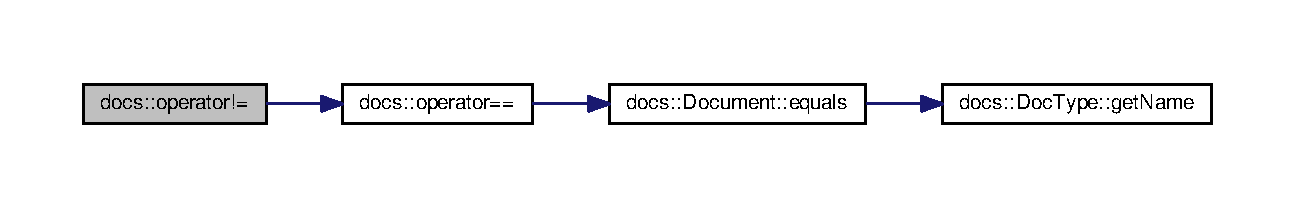
\includegraphics[width=350pt]{namespacedocs_abbb9bd3baf3e28ceb50a275bb0695e89_cgraph}
\end{center}
\end{figure}


\hypertarget{namespacedocs_a2464f4b0ad981aa2f4f4f56dd16afb18}{\index{docs@{docs}!operator$<$$<$@{operator$<$$<$}}
\index{operator$<$$<$@{operator$<$$<$}!docs@{docs}}
\subsubsection[{operator$<$$<$}]{\setlength{\rightskip}{0pt plus 5cm}std\-::ostream\& docs\-::operator$<$$<$ (
\begin{DoxyParamCaption}
\item[{std\-::ostream \&}]{strm, }
\item[{const Document \&}]{doc}
\end{DoxyParamCaption}
)}}\label{namespacedocs_a2464f4b0ad981aa2f4f4f56dd16afb18}
it returns 'strm $<$$<$ doc.\-to\-String()'. This method should not be implemented on derived classes. 

Definition at line 61 of file Document.\-cpp.



References docs\-::\-Document\-::to\-String().



Here is the call graph for this function\-:\nopagebreak
\begin{figure}[H]
\begin{center}
\leavevmode
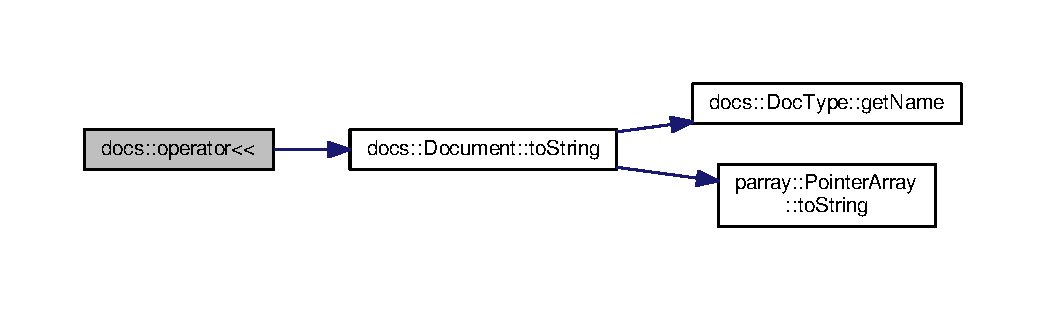
\includegraphics[width=350pt]{namespacedocs_a2464f4b0ad981aa2f4f4f56dd16afb18_cgraph}
\end{center}
\end{figure}


\hypertarget{namespacedocs_a69ecd221cb71a7f629bf48b283aefbc2}{\index{docs@{docs}!operator==@{operator==}}
\index{operator==@{operator==}!docs@{docs}}
\subsubsection[{operator==}]{\setlength{\rightskip}{0pt plus 5cm}bool docs\-::operator== (
\begin{DoxyParamCaption}
\item[{const Document \&}]{c1, }
\item[{const Document \&}]{c2}
\end{DoxyParamCaption}
)}}\label{namespacedocs_a69ecd221cb71a7f629bf48b283aefbc2}
it returns 'c1.\-equals( c2)'. This method should not be implemented on derived classes. 

Definition at line 84 of file Document.\-cpp.



References docs\-::\-Document\-::equals().



Referenced by operator!=().



Here is the call graph for this function\-:\nopagebreak
\begin{figure}[H]
\begin{center}
\leavevmode
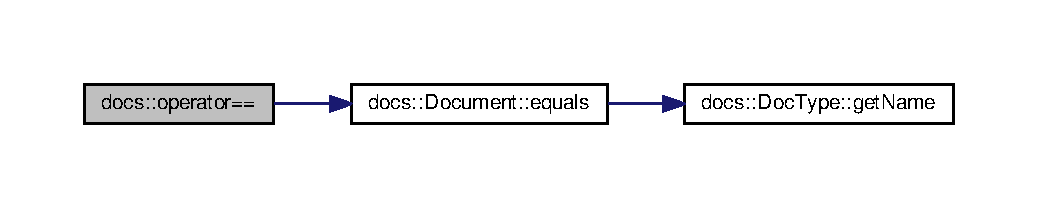
\includegraphics[width=350pt]{namespacedocs_a69ecd221cb71a7f629bf48b283aefbc2_cgraph}
\end{center}
\end{figure}



\hypertarget{namespaceparray}{\section{parray Namespace Reference}
\label{namespaceparray}\index{parray@{parray}}
}


it specify the dynamic array manager for a generic data T and a std\-::string specialisation.  


\subsection*{Classes}
\begin{DoxyCompactItemize}
\item 
class \hyperlink{classparray_1_1PointerArray}{Pointer\-Array}
\begin{DoxyCompactList}\small\item\em This class describes a manager of a dynamic array of generic type T$\ast$. \end{DoxyCompactList}\item 
class \hyperlink{classparray_1_1StringPointerArray}{String\-Pointer\-Array}
\begin{DoxyCompactList}\small\item\em It implements a \hyperlink{classparray_1_1PointerArray_ab506b284822d1e013813579e06893797}{Pointer\-Array} with a string parameter (T). \end{DoxyCompactList}\end{DoxyCompactItemize}
\subsection*{Variables}
\begin{DoxyCompactItemize}
\item 
\hypertarget{namespaceparray_ae12e5e44ecdf5808872ebdc05476e93f}{const std\-::string \hyperlink{namespaceparray_ae12e5e44ecdf5808872ebdc05476e93f}{L\-O\-G\-\_\-\-H\-E\-A\-D\-E\-R\-\_\-\-I\-N\-F\-O} = \char`\"{} Pointer\-Array\-: \char`\"{}}\label{namespaceparray_ae12e5e44ecdf5808872ebdc05476e93f}

\begin{DoxyCompactList}\small\item\em the debugging string to be appended on log head by this manager \end{DoxyCompactList}\item 
\hypertarget{namespaceparray_ab57bc1fd35280f9304abbf9755598710}{const std\-::string \hyperlink{namespaceparray_ab57bc1fd35280f9304abbf9755598710}{L\-O\-G\-\_\-\-H\-E\-A\-D\-E\-R\-\_\-\-T\-E\-S\-T} = \char`\"{}\textbackslash{}t\mbox{[}T\-E\-S\-T\mbox{]} \char`\"{} + L\-O\-G\-\_\-\-H\-E\-A\-D\-E\-R\-\_\-\-I\-N\-F\-O}\label{namespaceparray_ab57bc1fd35280f9304abbf9755598710}

\begin{DoxyCompactList}\small\item\em the debugging string to be appended on log head by the \hyperlink{classparray_1_1StringPointerArray_abfac13570bec8c88311714d19ddea59b}{String\-Pointer\-Array\-::tester()} \end{DoxyCompactList}\end{DoxyCompactItemize}


\subsection{Detailed Description}
it specify the dynamic array manager for a generic data T and a std\-::string specialisation. 
\hypertarget{namespacepatch}{\section{patch Namespace Reference}
\label{namespacepatch}\index{patch@{patch}}
}


to emulate C++11 and get to\-\_\-string translator  


\subsection*{Functions}
\begin{DoxyCompactItemize}
\item 
\hypertarget{namespacepatch_a54d2400c78aef13e3748a87cd7c86ede}{{\footnotesize template$<$typename T $>$ }\\std\-::string \hyperlink{namespacepatch_a54d2400c78aef13e3748a87cd7c86ede}{to\-\_\-string} (const T \&n)}\label{namespacepatch_a54d2400c78aef13e3748a87cd7c86ede}

\begin{DoxyCompactList}\small\item\em returns the description of the parameter by using $<$$<$ operator on a fresh std\-::ostringstream \end{DoxyCompactList}\end{DoxyCompactItemize}


\subsection{Detailed Description}
to emulate C++11 and get to\-\_\-string translator 
\chapter{Class Documentation}
\hypertarget{classdocs_1_1DocType}{\section{docs\-:\-:Doc\-Type Class Reference}
\label{classdocs_1_1DocType}\index{docs\-::\-Doc\-Type@{docs\-::\-Doc\-Type}}
}


The class containing the definition of \hyperlink{classdocs_1_1Document}{Document} Types names.  




{\ttfamily \#include $<$Document.\-h$>$}

\subsection*{Public Member Functions}
\begin{DoxyCompactItemize}
\item 
\hypertarget{classdocs_1_1DocType_a0ca0927d1a4d050487d9d14069afc050}{\hyperlink{classdocs_1_1DocType_a0ca0927d1a4d050487d9d14069afc050}{Doc\-Type} (\hyperlink{namespacedocs_a150efca62822b8ab62a5afabe299bf75}{Type} t)}\label{classdocs_1_1DocType_a0ca0927d1a4d050487d9d14069afc050}

\begin{DoxyCompactList}\small\item\em constructors must provide a final type to be attached on document constructors. \end{DoxyCompactList}\item 
\hypertarget{classdocs_1_1DocType_a931f25a0445c46eb7fba5c515124b728}{\hyperlink{classdocs_1_1DocType_a931f25a0445c46eb7fba5c515124b728}{$\sim$\-Doc\-Type} ()}\label{classdocs_1_1DocType_a931f25a0445c46eb7fba5c515124b728}

\begin{DoxyCompactList}\small\item\em empty since all instances of this class are suppose to be constant. \end{DoxyCompactList}\item 
\hypertarget{classdocs_1_1DocType_a1a7221ca7a1b44b1b115c81c469f6f75}{const \hyperlink{namespacedocs_a150efca62822b8ab62a5afabe299bf75}{Type} \hyperlink{classdocs_1_1DocType_a1a7221ca7a1b44b1b115c81c469f6f75}{get\-Type} () const }\label{classdocs_1_1DocType_a1a7221ca7a1b44b1b115c81c469f6f75}

\begin{DoxyCompactList}\small\item\em returns the final type I\-D. \end{DoxyCompactList}\item 
\hypertarget{classdocs_1_1DocType_a4632fc57ed71ebb984aa8dd78017db03}{const std\-::string \hyperlink{classdocs_1_1DocType_a4632fc57ed71ebb984aa8dd78017db03}{get\-Name} () const }\label{classdocs_1_1DocType_a4632fc57ed71ebb984aa8dd78017db03}

\begin{DoxyCompactList}\small\item\em returns the name of the type of the document and \char`\"{}\-Invalid Type\char`\"{} if unknown. \end{DoxyCompactList}\end{DoxyCompactItemize}
\subsection*{Friends}
\begin{DoxyCompactItemize}
\item 
\hypertarget{classdocs_1_1DocType_ab7f2e778c65c36835a714e77aa2c3a09}{std\-::ostream \& \hyperlink{classdocs_1_1DocType_ab7f2e778c65c36835a714e77aa2c3a09}{operator$<$$<$} (std\-::ostream \&st, const \hyperlink{classdocs_1_1DocType}{Doc\-Type} \&t)}\label{classdocs_1_1DocType_ab7f2e778c65c36835a714e77aa2c3a09}

\begin{DoxyCompactList}\small\item\em prints the \hyperlink{classdocs_1_1DocType_a4632fc57ed71ebb984aa8dd78017db03}{get\-Name()} result. \end{DoxyCompactList}\item 
\hypertarget{classdocs_1_1DocType_aa68c01dc0d9b0494723b223bf52a6acf}{bool \hyperlink{classdocs_1_1DocType_aa68c01dc0d9b0494723b223bf52a6acf}{operator==} (const \hyperlink{classdocs_1_1DocType}{Doc\-Type} \&c1, const \hyperlink{classdocs_1_1DocType}{Doc\-Type} \&c2)}\label{classdocs_1_1DocType_aa68c01dc0d9b0494723b223bf52a6acf}

\begin{DoxyCompactList}\small\item\em return the comparison of \hyperlink{classdocs_1_1DocType_a4632fc57ed71ebb984aa8dd78017db03}{get\-Name()} methods. \end{DoxyCompactList}\item 
\hypertarget{classdocs_1_1DocType_a6f7b8c51d3dc0ec95808119766eb8010}{bool \hyperlink{classdocs_1_1DocType_a6f7b8c51d3dc0ec95808119766eb8010}{operator!=} (const \hyperlink{classdocs_1_1DocType}{Doc\-Type} \&c1, const \hyperlink{classdocs_1_1DocType}{Doc\-Type} \&c2)}\label{classdocs_1_1DocType_a6f7b8c51d3dc0ec95808119766eb8010}

\begin{DoxyCompactList}\small\item\em return the negation of the comparison of \hyperlink{classdocs_1_1DocType_a4632fc57ed71ebb984aa8dd78017db03}{get\-Name()}. \end{DoxyCompactList}\end{DoxyCompactItemize}


\subsection{Detailed Description}
The class containing the definition of \hyperlink{classdocs_1_1Document}{Document} Types names. 

\begin{DoxySeeAlso}{See Also}
\hyperlink{namespacedocs_a150efca62822b8ab62a5afabe299bf75}{Type} 

\hyperlink{namespacedocs_a88f8e41b03147cf4197261676999d12c}{T\-Y\-P\-E\-\_\-\-N\-A\-M\-E\-\_\-\-D\-O\-C\-U\-M\-E\-N\-T} 

\hyperlink{namespacedocs_ac41cf3635e22c3750deddd000fd4c34b}{T\-Y\-P\-E\-\_\-\-N\-A\-M\-E\-\_\-\-W\-E\-B\-P\-A\-G\-E} 

\hyperlink{namespacedocs_a3f58481f03c01b3da04828585d14ff77}{T\-Y\-P\-E\-\_\-\-N\-A\-M\-E\-\_\-\-S\-P\-R\-E\-A\-D\-S\-H\-E\-E\-T}
\end{DoxySeeAlso}
It allows to print the name of the of type of document and at the same time make an easy comparison or perhaps a searching rule. 

Definition at line 84 of file Document.\-h.



The documentation for this class was generated from the following file\-:\begin{DoxyCompactItemize}
\item 
src/\hyperlink{Document_8h}{Document.\-h}\end{DoxyCompactItemize}

\hypertarget{classdocs_1_1Document}{\section{docs\-:\-:Document Class Reference}
\label{classdocs_1_1Document}\index{docs\-::\-Document@{docs\-::\-Document}}
}


This is the base class of the \hyperlink{classdocs_1_1Document}{Document} hierarchy.  




{\ttfamily \#include $<$Document.\-h$>$}



Inheritance diagram for docs\-:\-:Document\-:\nopagebreak
\begin{figure}[H]
\begin{center}
\leavevmode
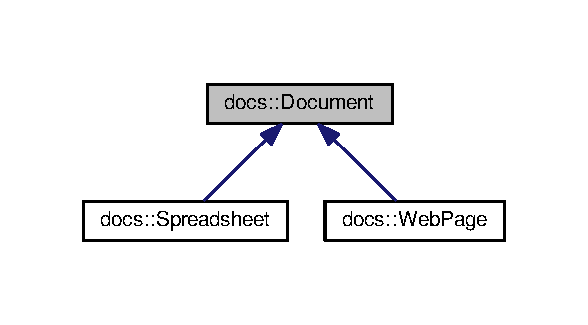
\includegraphics[width=282pt]{classdocs_1_1Document__inherit__graph}
\end{center}
\end{figure}


Collaboration diagram for docs\-:\-:Document\-:\nopagebreak
\begin{figure}[H]
\begin{center}
\leavevmode
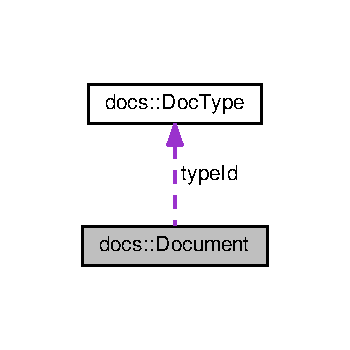
\includegraphics[width=309pt]{classdocs_1_1Document__coll__graph}
\end{center}
\end{figure}
\subsection*{Public Member Functions}
\begin{DoxyCompactItemize}
\item 
\hypertarget{classdocs_1_1Document_ace8d18f691181e1676a6ca5207da336b}{\hyperlink{classdocs_1_1Document_ace8d18f691181e1676a6ca5207da336b}{Document} (std\-::string \hyperlink{classdocs_1_1Document_a419e4470c20e1bddd60448ba430f4738}{title}=\hyperlink{namespacedocs_a4cf6dd6732c7e7ab7f7855e440485d89}{D\-E\-F\-A\-U\-L\-T\-\_\-\-D\-O\-C\-U\-M\-E\-N\-T\-\_\-\-T\-I\-T\-L\-E}, int key\-Word\-Size=\hyperlink{namespacedocs_ae635b9481a61628036b5a97625856475}{D\-E\-F\-A\-U\-L\-T\-\_\-\-D\-O\-C\-U\-M\-E\-N\-T\-\_\-\-K\-W\-S\-I\-Z\-E})}\label{classdocs_1_1Document_ace8d18f691181e1676a6ca5207da336b}

\begin{DoxyCompactList}\small\item\em construct by creating a new keyword list. \end{DoxyCompactList}\item 
\hypertarget{classdocs_1_1Document_aa9c1a4e9b6aab58e8e28b16a2888e601}{\hyperlink{classdocs_1_1Document_aa9c1a4e9b6aab58e8e28b16a2888e601}{Document} (const \hyperlink{classparray_1_1StringPointerArray}{parray\-::\-String\-Pointer\-Array} \&kws, std\-::string \hyperlink{classdocs_1_1Document_a419e4470c20e1bddd60448ba430f4738}{title}=\hyperlink{namespacedocs_a4cf6dd6732c7e7ab7f7855e440485d89}{D\-E\-F\-A\-U\-L\-T\-\_\-\-D\-O\-C\-U\-M\-E\-N\-T\-\_\-\-T\-I\-T\-L\-E})}\label{classdocs_1_1Document_aa9c1a4e9b6aab58e8e28b16a2888e601}

\begin{DoxyCompactList}\small\item\em construct by using a copy of a Pointer\-Array of string. \end{DoxyCompactList}\item 
\hypertarget{classdocs_1_1Document_ad65291ea47b0be5a29d2ba13868a8a7c}{\hyperlink{classdocs_1_1Document_ad65291ea47b0be5a29d2ba13868a8a7c}{Document} (const \hyperlink{classdocs_1_1Document}{Document} \&original)}\label{classdocs_1_1Document_ad65291ea47b0be5a29d2ba13868a8a7c}

\begin{DoxyCompactList}\small\item\em \hyperlink{classdocs_1_1Document_ad8b6a91c7a8e39a880790d14aba14322}{copy()} constructor, to create an independent clone. \end{DoxyCompactList}\item 
\hypertarget{classdocs_1_1Document_abcb73ac5ddf4e7b0c862220228b85b9e}{virtual \hyperlink{classdocs_1_1Document_abcb73ac5ddf4e7b0c862220228b85b9e}{$\sim$\-Document} ()}\label{classdocs_1_1Document_abcb73ac5ddf4e7b0c862220228b85b9e}

\begin{DoxyCompactList}\small\item\em destructor, to clear the keywords list. \end{DoxyCompactList}\item 
\hypertarget{classdocs_1_1Document_ad7026f3128f00be0e80bb9dc7d220da4}{\hyperlink{classdocs_1_1Document}{Document} \& \hyperlink{classdocs_1_1Document_ad7026f3128f00be0e80bb9dc7d220da4}{operator=} (const \hyperlink{classdocs_1_1Document}{Document} \&)}\label{classdocs_1_1Document_ad7026f3128f00be0e80bb9dc7d220da4}

\begin{DoxyCompactList}\small\item\em to \hyperlink{classdocs_1_1Document_ad8b6a91c7a8e39a880790d14aba14322}{copy()} this object \end{DoxyCompactList}\item 
\hypertarget{classdocs_1_1Document_a16db383045038b779eb489ad125ef02b}{virtual const std\-::string \hyperlink{classdocs_1_1Document_a16db383045038b779eb489ad125ef02b}{to\-String} () const }\label{classdocs_1_1Document_a16db383045038b779eb489ad125ef02b}

\begin{DoxyCompactList}\small\item\em print the information of this object by listing all the data members. \end{DoxyCompactList}\item 
\hypertarget{classdocs_1_1Document_ad86b3a7c7d496f3b05c740e2c1433c78}{virtual bool const \hyperlink{classdocs_1_1Document_ad86b3a7c7d496f3b05c740e2c1433c78}{equals} (const \hyperlink{classdocs_1_1Document}{Document} \&) const }\label{classdocs_1_1Document_ad86b3a7c7d496f3b05c740e2c1433c78}

\begin{DoxyCompactList}\small\item\em check if all the data member are equals (type, title, key\-Words). \end{DoxyCompactList}\item 
\hypertarget{classdocs_1_1Document_a06b90f239984c69784c877d670943fb5}{virtual std\-::string \hyperlink{classdocs_1_1Document_a06b90f239984c69784c877d670943fb5}{get\-Title} () const }\label{classdocs_1_1Document_a06b90f239984c69784c877d670943fb5}

\begin{DoxyCompactList}\small\item\em return the \hyperlink{classdocs_1_1Document_a419e4470c20e1bddd60448ba430f4738}{title} of this document \end{DoxyCompactList}\item 
\hypertarget{classdocs_1_1Document_afdf0fd42a3afe3c7c2523b3ee16d09e0}{virtual void \hyperlink{classdocs_1_1Document_afdf0fd42a3afe3c7c2523b3ee16d09e0}{set\-Title} (const std\-::string)}\label{classdocs_1_1Document_afdf0fd42a3afe3c7c2523b3ee16d09e0}

\begin{DoxyCompactList}\small\item\em set a \hyperlink{classdocs_1_1Document_a419e4470c20e1bddd60448ba430f4738}{title} to this document. \end{DoxyCompactList}\item 
\hypertarget{classdocs_1_1Document_a500da2818240e2b29c1e4510b8724f4f}{virtual \\*
\hyperlink{classparray_1_1StringPointerArray}{parray\-::\-String\-Pointer\-Array} $\ast$ \hyperlink{classdocs_1_1Document_a500da2818240e2b29c1e4510b8724f4f}{get\-Key\-Words} () const }\label{classdocs_1_1Document_a500da2818240e2b29c1e4510b8724f4f}

\begin{DoxyCompactList}\small\item\em returns the manager of the \hyperlink{classdocs_1_1Document_a7539ac1430ded1f3a15f2532de8f0381}{key\-Words} array of this document. \end{DoxyCompactList}\item 
\hypertarget{classdocs_1_1Document_a99cde56ac7b8b230184b938cf55ce17e}{virtual void \hyperlink{classdocs_1_1Document_a99cde56ac7b8b230184b938cf55ce17e}{set\-Key\-Words} (\hyperlink{classparray_1_1StringPointerArray}{parray\-::\-String\-Pointer\-Array} $\ast$)}\label{classdocs_1_1Document_a99cde56ac7b8b230184b938cf55ce17e}

\begin{DoxyCompactList}\small\item\em set a copy of the input \hyperlink{classdocs_1_1Document_a7539ac1430ded1f3a15f2532de8f0381}{key\-Words} and overwrites the previous. \end{DoxyCompactList}\item 
\hypertarget{classdocs_1_1Document_a9b7139734ec394970161695e2e06c263}{virtual const std\-::string $\ast$ \hyperlink{classdocs_1_1Document_a9b7139734ec394970161695e2e06c263}{get\-Key\-Words\-Array} () const }\label{classdocs_1_1Document_a9b7139734ec394970161695e2e06c263}

\begin{DoxyCompactList}\small\item\em returns the dynamic array containing the \hyperlink{classdocs_1_1Document_a7539ac1430ded1f3a15f2532de8f0381}{key\-Words} \end{DoxyCompactList}\item 
\hypertarget{classdocs_1_1Document_a0af7d404eb347f27bc4e42b085aaa038}{virtual const int \hyperlink{classdocs_1_1Document_a0af7d404eb347f27bc4e42b085aaa038}{get\-Key\-Words\-Size} () const }\label{classdocs_1_1Document_a0af7d404eb347f27bc4e42b085aaa038}

\begin{DoxyCompactList}\small\item\em returns the \hyperlink{classdocs_1_1Document_a9b7139734ec394970161695e2e06c263}{get\-Key\-Words\-Array()} size \end{DoxyCompactList}\item 
\hypertarget{classdocs_1_1Document_a5626bdb2863afb9c3dd363fc5cc1bbde}{const \hyperlink{classdocs_1_1DocType}{Doc\-Type} \hyperlink{classdocs_1_1Document_a5626bdb2863afb9c3dd363fc5cc1bbde}{get\-Type} () const }\label{classdocs_1_1Document_a5626bdb2863afb9c3dd363fc5cc1bbde}

\begin{DoxyCompactList}\small\item\em return the type identifier of this document assigned on custruction. \end{DoxyCompactList}\end{DoxyCompactItemize}
\subsection*{Protected Member Functions}
\begin{DoxyCompactItemize}
\item 
\hypertarget{classdocs_1_1Document_ad8b6a91c7a8e39a880790d14aba14322}{virtual void \hyperlink{classdocs_1_1Document_ad8b6a91c7a8e39a880790d14aba14322}{copy} (const \hyperlink{classdocs_1_1Document}{Document} \&)}\label{classdocs_1_1Document_ad8b6a91c7a8e39a880790d14aba14322}

\begin{DoxyCompactList}\small\item\em copy this object on a new memory location. \end{DoxyCompactList}\item 
\hypertarget{classdocs_1_1Document_a9f0b2c4c1a3e3344f374330399969e90}{\hyperlink{classdocs_1_1Document_a9f0b2c4c1a3e3344f374330399969e90}{Document} (const \hyperlink{classdocs_1_1DocType}{Doc\-Type} \hyperlink{classdocs_1_1Document_ad5250ef4bd98928dfbe6243162536389}{type\-Id}, const std\-::string \hyperlink{classdocs_1_1Document_a419e4470c20e1bddd60448ba430f4738}{title}=\hyperlink{namespacedocs_a4cf6dd6732c7e7ab7f7855e440485d89}{D\-E\-F\-A\-U\-L\-T\-\_\-\-D\-O\-C\-U\-M\-E\-N\-T\-\_\-\-T\-I\-T\-L\-E}, const int key\-Word\-Size=\hyperlink{namespacedocs_ae635b9481a61628036b5a97625856475}{D\-E\-F\-A\-U\-L\-T\-\_\-\-D\-O\-C\-U\-M\-E\-N\-T\-\_\-\-K\-W\-S\-I\-Z\-E})}\label{classdocs_1_1Document_a9f0b2c4c1a3e3344f374330399969e90}

\begin{DoxyCompactList}\small\item\em The \hyperlink{classdocs_1_1Document_ace8d18f691181e1676a6ca5207da336b}{Document( std\-::string, int)} constructor to be use on derived class for specifying the document type\-Id I\-D. \end{DoxyCompactList}\item 
\hypertarget{classdocs_1_1Document_a4a76d0cee2709582e4b9f3b5b8db0277}{\hyperlink{classdocs_1_1Document_a4a76d0cee2709582e4b9f3b5b8db0277}{Document} (const \hyperlink{classdocs_1_1DocType}{Doc\-Type} \hyperlink{classdocs_1_1Document_ad5250ef4bd98928dfbe6243162536389}{type\-Id}, const \hyperlink{classparray_1_1StringPointerArray}{parray\-::\-String\-Pointer\-Array} \&kws, const std\-::string \hyperlink{classdocs_1_1Document_a419e4470c20e1bddd60448ba430f4738}{title}=\hyperlink{namespacedocs_a4cf6dd6732c7e7ab7f7855e440485d89}{D\-E\-F\-A\-U\-L\-T\-\_\-\-D\-O\-C\-U\-M\-E\-N\-T\-\_\-\-T\-I\-T\-L\-E})}\label{classdocs_1_1Document_a4a76d0cee2709582e4b9f3b5b8db0277}

\begin{DoxyCompactList}\small\item\em The \hyperlink{classdocs_1_1Document_aa9c1a4e9b6aab58e8e28b16a2888e601}{Document( const parray\-::\-String\-Pointer\-Array\&, std\-::string)} constructor to be use on derived class for specifying the document type\-Id I\-D. \end{DoxyCompactList}\end{DoxyCompactItemize}
\subsection*{Protected Attributes}
\begin{DoxyCompactItemize}
\item 
\hypertarget{classdocs_1_1Document_ad5250ef4bd98928dfbe6243162536389}{const \hyperlink{classdocs_1_1DocType}{Doc\-Type} \hyperlink{classdocs_1_1Document_ad5250ef4bd98928dfbe6243162536389}{type\-Id}}\label{classdocs_1_1Document_ad5250ef4bd98928dfbe6243162536389}

\begin{DoxyCompactList}\small\item\em the type I\-D assigned to this document on constructor. \end{DoxyCompactList}\end{DoxyCompactItemize}
\subsection*{Private Attributes}
\begin{DoxyCompactItemize}
\item 
\hypertarget{classdocs_1_1Document_a419e4470c20e1bddd60448ba430f4738}{std\-::string \hyperlink{classdocs_1_1Document_a419e4470c20e1bddd60448ba430f4738}{title}}\label{classdocs_1_1Document_a419e4470c20e1bddd60448ba430f4738}

\begin{DoxyCompactList}\small\item\em the title of this \hyperlink{classdocs_1_1Document}{Document}. \end{DoxyCompactList}\item 
\hypertarget{classdocs_1_1Document_a7539ac1430ded1f3a15f2532de8f0381}{\hyperlink{classparray_1_1StringPointerArray}{parray\-::\-String\-Pointer\-Array} $\ast$ \hyperlink{classdocs_1_1Document_a7539ac1430ded1f3a15f2532de8f0381}{key\-Words}}\label{classdocs_1_1Document_a7539ac1430ded1f3a15f2532de8f0381}

\begin{DoxyCompactList}\small\item\em the key word array manager of this \hyperlink{classdocs_1_1Document}{Document}. \end{DoxyCompactList}\end{DoxyCompactItemize}
\subsection*{Friends}
\begin{DoxyCompactItemize}
\item 
std\-::ostream \& \hyperlink{classdocs_1_1Document_a801e6c851261e550881c632d31407c55}{operator$<$$<$} (std\-::ostream \&, const \hyperlink{classdocs_1_1Document}{Document} \&)
\begin{DoxyCompactList}\small\item\em return the result of \hyperlink{classdocs_1_1Document_a16db383045038b779eb489ad125ef02b}{to\-String()}. \end{DoxyCompactList}\item 
bool \hyperlink{classdocs_1_1Document_aba6a95005cddfc7e9b668de3b0160cc6}{operator==} (const \hyperlink{classdocs_1_1Document}{Document} \&, const \hyperlink{classdocs_1_1Document}{Document} \&)
\begin{DoxyCompactList}\small\item\em returns the result of \hyperlink{classdocs_1_1Document_ad86b3a7c7d496f3b05c740e2c1433c78}{equals()}. \end{DoxyCompactList}\item 
bool \hyperlink{classdocs_1_1Document_abda12a8e6c13277b760c0e40efa44695}{operator!=} (const \hyperlink{classdocs_1_1Document}{Document} \&, const \hyperlink{classdocs_1_1Document}{Document} \&)
\begin{DoxyCompactList}\small\item\em returns the negation of \hyperlink{classdocs_1_1Document_ad86b3a7c7d496f3b05c740e2c1433c78}{equals()} \end{DoxyCompactList}\end{DoxyCompactItemize}


\subsection{Detailed Description}
This is the base class of the \hyperlink{classdocs_1_1Document}{Document} hierarchy. 

\begin{DoxySeeAlso}{See Also}
\hyperlink{classdocs_1_1DocType}{Doc\-Type} 

\hyperlink{classparray_1_1StringPointerArray}{parray\-::\-String\-Pointer\-Array}
\end{DoxySeeAlso}
It describes a generic document through\-: a Type, a title (string) and a keyword set (Pointer\-Array). It implements default empty and copy constructors as well as basic operator overloading. 

\subsection{Friends And Related Function Documentation}
\hypertarget{classdocs_1_1Document_abda12a8e6c13277b760c0e40efa44695}{\index{docs\-::\-Document@{docs\-::\-Document}!operator!=@{operator!=}}
\index{operator!=@{operator!=}!docs::Document@{docs\-::\-Document}}
\subsubsection[{operator!=}]{\setlength{\rightskip}{0pt plus 5cm}bool operator!= (
\begin{DoxyParamCaption}
\item[{const {\bf Document} \&}]{c1, }
\item[{const {\bf Document} \&}]{c2}
\end{DoxyParamCaption}
)\hspace{0.3cm}{\ttfamily [friend]}}}\label{classdocs_1_1Document_abda12a8e6c13277b760c0e40efa44695}


returns the negation of \hyperlink{classdocs_1_1Document_ad86b3a7c7d496f3b05c740e2c1433c78}{equals()} 

it returns '!c1.equals( c2)'. This method should not be implemented on derived classes. \hypertarget{classdocs_1_1Document_a801e6c851261e550881c632d31407c55}{\index{docs\-::\-Document@{docs\-::\-Document}!operator$<$$<$@{operator$<$$<$}}
\index{operator$<$$<$@{operator$<$$<$}!docs::Document@{docs\-::\-Document}}
\subsubsection[{operator$<$$<$}]{\setlength{\rightskip}{0pt plus 5cm}std\-::ostream\& operator$<$$<$ (
\begin{DoxyParamCaption}
\item[{std\-::ostream \&}]{strm, }
\item[{const {\bf Document} \&}]{doc}
\end{DoxyParamCaption}
)\hspace{0.3cm}{\ttfamily [friend]}}}\label{classdocs_1_1Document_a801e6c851261e550881c632d31407c55}


return the result of \hyperlink{classdocs_1_1Document_a16db383045038b779eb489ad125ef02b}{to\-String()}. 

it returns 'strm $<$$<$ doc.\-to\-String()'. This method should not be implemented on derived classes. \hypertarget{classdocs_1_1Document_aba6a95005cddfc7e9b668de3b0160cc6}{\index{docs\-::\-Document@{docs\-::\-Document}!operator==@{operator==}}
\index{operator==@{operator==}!docs::Document@{docs\-::\-Document}}
\subsubsection[{operator==}]{\setlength{\rightskip}{0pt plus 5cm}bool operator== (
\begin{DoxyParamCaption}
\item[{const {\bf Document} \&}]{c1, }
\item[{const {\bf Document} \&}]{c2}
\end{DoxyParamCaption}
)\hspace{0.3cm}{\ttfamily [friend]}}}\label{classdocs_1_1Document_aba6a95005cddfc7e9b668de3b0160cc6}


returns the result of \hyperlink{classdocs_1_1Document_ad86b3a7c7d496f3b05c740e2c1433c78}{equals()}. 

it returns 'c1.\-equals( c2)'. This method should not be implemented on derived classes. 

The documentation for this class was generated from the following files\-:\begin{DoxyCompactItemize}
\item 
src/\hyperlink{Document_8h}{Document.\-h}\item 
src/\hyperlink{Document_8cpp}{Document.\-cpp}\end{DoxyCompactItemize}

\hypertarget{classparray_1_1PointerArray}{\section{parray\-:\-:Pointer\-Array$<$ T $>$ Class Template Reference}
\label{classparray_1_1PointerArray}\index{parray\-::\-Pointer\-Array$<$ T $>$@{parray\-::\-Pointer\-Array$<$ T $>$}}
}


This class describes a manager of a dynamic array of generic type T$\ast$.  


\subsection*{Public Member Functions}
\begin{DoxyCompactItemize}
\item 
\hypertarget{classparray_1_1PointerArray_ab506b284822d1e013813579e06893797}{\hyperlink{classparray_1_1PointerArray_ab506b284822d1e013813579e06893797}{Pointer\-Array} ()}\label{classparray_1_1PointerArray_ab506b284822d1e013813579e06893797}

\begin{DoxyCompactList}\small\item\em does not initialise the set and invalidates the counter (generates also warning log to advertise the call of \hyperlink{classparray_1_1PointerArray_ae3fb455ddc80180a3a7b130cb2c4d903}{set\-Size()}) \end{DoxyCompactList}\item 
\hypertarget{classparray_1_1PointerArray_a4e39d7adf15e94c02dfe2662c181f0c6}{\hyperlink{classparray_1_1PointerArray_a4e39d7adf15e94c02dfe2662c181f0c6}{Pointer\-Array} (const int length)}\label{classparray_1_1PointerArray_a4e39d7adf15e94c02dfe2662c181f0c6}

\begin{DoxyCompactList}\small\item\em create a new empty array of specified size \end{DoxyCompactList}\item 
\hypertarget{classparray_1_1PointerArray_ab763be75c142552337e545ca0a27d93e}{\hyperlink{classparray_1_1PointerArray_ab763be75c142552337e545ca0a27d93e}{Pointer\-Array} (const \hyperlink{classparray_1_1PointerArray}{Pointer\-Array}$<$ T $>$ \&original)}\label{classparray_1_1PointerArray_ab763be75c142552337e545ca0a27d93e}

\begin{DoxyCompactList}\small\item\em \#copy() constructors \end{DoxyCompactList}\item 
\hypertarget{classparray_1_1PointerArray_a3b59a3fe4f7e83d83231d9daf8210333}{virtual \hyperlink{classparray_1_1PointerArray_a3b59a3fe4f7e83d83231d9daf8210333}{$\sim$\-Pointer\-Array} ()}\label{classparray_1_1PointerArray_a3b59a3fe4f7e83d83231d9daf8210333}

\begin{DoxyCompactList}\small\item\em destructors, invalidate counter, pointer and clear memory. Logs\-: \char`\"{}deleting\char`\"{}, for debugging purposes. \end{DoxyCompactList}\item 
\hypertarget{classparray_1_1PointerArray_ae3fb455ddc80180a3a7b130cb2c4d903}{void \hyperlink{classparray_1_1PointerArray_ae3fb455ddc80180a3a7b130cb2c4d903}{set\-Size} (const int length)}\label{classparray_1_1PointerArray_ae3fb455ddc80180a3a7b130cb2c4d903}

\begin{DoxyCompactList}\small\item\em set the size of a new empty array on memory and delete the previous. \end{DoxyCompactList}\item 
\hypertarget{classparray_1_1PointerArray_ac676a9ef1cc04a9aab5f9b744142bf61}{int \hyperlink{classparray_1_1PointerArray_ac676a9ef1cc04a9aab5f9b744142bf61}{get\-Size} () const }\label{classparray_1_1PointerArray_ac676a9ef1cc04a9aab5f9b744142bf61}

\begin{DoxyCompactList}\small\item\em returns the actual size of the array. \end{DoxyCompactList}\item 
\hypertarget{classparray_1_1PointerArray_ac6ad9597cf9fb62857a143e3c241223e}{int \hyperlink{classparray_1_1PointerArray_ac6ad9597cf9fb62857a143e3c241223e}{get\-Cnt} () const }\label{classparray_1_1PointerArray_ac6ad9597cf9fb62857a143e3c241223e}

\begin{DoxyCompactList}\small\item\em returns the actual number of elements in the array. \end{DoxyCompactList}\item 
\hypertarget{classparray_1_1PointerArray_ac2fc7fd12afb0d8fa908ad02a3e39d28}{const T $\ast$ \hyperlink{classparray_1_1PointerArray_ac2fc7fd12afb0d8fa908ad02a3e39d28}{get\-Array} () const }\label{classparray_1_1PointerArray_ac2fc7fd12afb0d8fa908ad02a3e39d28}

\begin{DoxyCompactList}\small\item\em returns the head to the memory managed by this class. \end{DoxyCompactList}\item 
\hypertarget{classparray_1_1PointerArray_a97dbb10226a33da7823685fafe609194}{virtual const T \& \hyperlink{classparray_1_1PointerArray_a97dbb10226a33da7823685fafe609194}{get} (int idx) const }\label{classparray_1_1PointerArray_a97dbb10226a33da7823685fafe609194}

\begin{DoxyCompactList}\small\item\em returns an element of the array by index. \end{DoxyCompactList}\item 
const T \& \hyperlink{classparray_1_1PointerArray_aa009614c6819fe08b7eef78be4394dbc}{operator\mbox{[}$\,$\mbox{]}} (size\-\_\-t idx) const 
\item 
\hypertarget{classparray_1_1PointerArray_ae080aeced3af072006e4a609fdadb838}{virtual bool \hyperlink{classparray_1_1PointerArray_ae080aeced3af072006e4a609fdadb838}{add} (const T to\-Add)}\label{classparray_1_1PointerArray_ae080aeced3af072006e4a609fdadb838}

\begin{DoxyCompactList}\small\item\em add an element into the array. Returns false if the array is full \end{DoxyCompactList}\item 
\hypertarget{classparray_1_1PointerArray_a436b6664985dbe49c1a70c2ed79573b3}{virtual const int \hyperlink{classparray_1_1PointerArray_a436b6664985dbe49c1a70c2ed79573b3}{find} (const T to\-Find) const }\label{classparray_1_1PointerArray_a436b6664985dbe49c1a70c2ed79573b3}

\begin{DoxyCompactList}\small\item\em returns the index of an occurrence in the array. -\/1 if not found \end{DoxyCompactList}\item 
\hypertarget{classparray_1_1PointerArray_a2c61803a24765673a1f59ba194566946}{virtual void \hyperlink{classparray_1_1PointerArray_a2c61803a24765673a1f59ba194566946}{clear} ()}\label{classparray_1_1PointerArray_a2c61803a24765673a1f59ba194566946}

\begin{DoxyCompactList}\small\item\em delete the array and create a new memory location of the same size. \end{DoxyCompactList}\item 
\hypertarget{classparray_1_1PointerArray_a13ae3b9b2118416351cc63bd456ecf73}{virtual const bool \hyperlink{classparray_1_1PointerArray_a13ae3b9b2118416351cc63bd456ecf73}{remove} (T to\-Remove)}\label{classparray_1_1PointerArray_a13ae3b9b2118416351cc63bd456ecf73}

\begin{DoxyCompactList}\small\item\em remove an element from the array (based on \hyperlink{classparray_1_1PointerArray_a436b6664985dbe49c1a70c2ed79573b3}{find()} and \hyperlink{classparray_1_1PointerArray_a803f8433e144a60f93e61afc7028d423}{remove(int)}). \end{DoxyCompactList}\item 
\hypertarget{classparray_1_1PointerArray_a803f8433e144a60f93e61afc7028d423}{virtual const bool \hyperlink{classparray_1_1PointerArray_a803f8433e144a60f93e61afc7028d423}{remove} (int idx)}\label{classparray_1_1PointerArray_a803f8433e144a60f93e61afc7028d423}

\begin{DoxyCompactList}\small\item\em remove an element from the array by index. \end{DoxyCompactList}\item 
\hypertarget{classparray_1_1PointerArray_a6d4347a899d2783d23775957ad71f743}{virtual void \hyperlink{classparray_1_1PointerArray_a6d4347a899d2783d23775957ad71f743}{resize} (const int new\-Lenght)}\label{classparray_1_1PointerArray_a6d4347a899d2783d23775957ad71f743}

\begin{DoxyCompactList}\small\item\em replace the array with a new memory of the defined size. Possible old values are copied from start up to fill the array. \end{DoxyCompactList}\item 
\hypertarget{classparray_1_1PointerArray_a13883fc7ef994a50a83ae3f9ddc4db27}{virtual void \hyperlink{classparray_1_1PointerArray_a13883fc7ef994a50a83ae3f9ddc4db27}{pack} ()}\label{classparray_1_1PointerArray_a13883fc7ef994a50a83ae3f9ddc4db27}

\begin{DoxyCompactList}\small\item\em replace the array by removing empty cell on tail (size will be equal to cnt). Based on \hyperlink{classparray_1_1PointerArray_a6d4347a899d2783d23775957ad71f743}{resize()}. \end{DoxyCompactList}\item 
\hypertarget{classparray_1_1PointerArray_a4c6e34cad01f5f72dd6c5de917ed3a34}{virtual const std\-::string \hyperlink{classparray_1_1PointerArray_a4c6e34cad01f5f72dd6c5de917ed3a34}{to\-String} () const }\label{classparray_1_1PointerArray_a4c6e34cad01f5f72dd6c5de917ed3a34}

\begin{DoxyCompactList}\small\item\em returns a description of the memory managed by this class \end{DoxyCompactList}\item 
\hypertarget{classparray_1_1PointerArray_a2ca07f329b7568d2bdd4ea50ba153a2b}{virtual bool \hyperlink{classparray_1_1PointerArray_a2ca07f329b7568d2bdd4ea50ba153a2b}{equals} (const \hyperlink{classparray_1_1PointerArray}{Pointer\-Array}$<$ T $>$ \&to\-Compare) const }\label{classparray_1_1PointerArray_a2ca07f329b7568d2bdd4ea50ba153a2b}

\begin{DoxyCompactList}\small\item\em returns true if all the elements of this array are the only elements of the parameter. \end{DoxyCompactList}\item 
\hypertarget{classparray_1_1PointerArray_acc9c164599807ed762727667f6b6bf13}{\hyperlink{classparray_1_1PointerArray}{Pointer\-Array}$<$ T $>$ \& \hyperlink{classparray_1_1PointerArray_acc9c164599807ed762727667f6b6bf13}{operator=} (const \hyperlink{classparray_1_1PointerArray}{Pointer\-Array}$<$ T $>$ \&new\-Copy)}\label{classparray_1_1PointerArray_acc9c164599807ed762727667f6b6bf13}

\begin{DoxyCompactList}\small\item\em make a \#copy() of this array. \end{DoxyCompactList}\item 
\hypertarget{classparray_1_1PointerArray_adf7c87ef3e5b66d11137209d45701975}{virtual const bool \hyperlink{classparray_1_1PointerArray_adf7c87ef3e5b66d11137209d45701975}{is\-Empty} () const }\label{classparray_1_1PointerArray_adf7c87ef3e5b66d11137209d45701975}

\begin{DoxyCompactList}\small\item\em returns true if there are no elements in the array. \end{DoxyCompactList}\item 
\hypertarget{classparray_1_1PointerArray_ac1aa766707215ddeecbf23a0648644c5}{bool const \hyperlink{classparray_1_1PointerArray_ac1aa766707215ddeecbf23a0648644c5}{operator!} () const }\label{classparray_1_1PointerArray_ac1aa766707215ddeecbf23a0648644c5}

\begin{DoxyCompactList}\small\item\em returns \hyperlink{classparray_1_1PointerArray_adf7c87ef3e5b66d11137209d45701975}{is\-Empty()}. \end{DoxyCompactList}\end{DoxyCompactItemize}
\subsection*{Friends}
\begin{DoxyCompactItemize}
\item 
\hypertarget{classparray_1_1PointerArray_a081ebddab3580154920d0739f567551d}{std\-::ostream \& \hyperlink{classparray_1_1PointerArray_a081ebddab3580154920d0739f567551d}{operator$<$$<$} (std\-::ostream \&strm, const \hyperlink{classparray_1_1PointerArray}{Pointer\-Array}$<$ T $>$ \&par)}\label{classparray_1_1PointerArray_a081ebddab3580154920d0739f567551d}

\begin{DoxyCompactList}\small\item\em calls \hyperlink{classparray_1_1PointerArray_a4c6e34cad01f5f72dd6c5de917ed3a34}{to\-String()} to describe the object. \end{DoxyCompactList}\item 
\hypertarget{classparray_1_1PointerArray_a050d55aeebf51f02bf59d8352664528d}{bool \hyperlink{classparray_1_1PointerArray_a050d55aeebf51f02bf59d8352664528d}{operator==} (const \hyperlink{classparray_1_1PointerArray}{Pointer\-Array}$<$ T $>$ \&c1, const \hyperlink{classparray_1_1PointerArray}{Pointer\-Array}$<$ T $>$ \&c2)}\label{classparray_1_1PointerArray_a050d55aeebf51f02bf59d8352664528d}

\begin{DoxyCompactList}\small\item\em calls \hyperlink{classparray_1_1PointerArray_a2ca07f329b7568d2bdd4ea50ba153a2b}{equals()} \end{DoxyCompactList}\item 
\hypertarget{classparray_1_1PointerArray_a8ef9d256b362ccc682a1ad998f92beda}{bool \hyperlink{classparray_1_1PointerArray_a8ef9d256b362ccc682a1ad998f92beda}{operator!=} (const \hyperlink{classparray_1_1PointerArray}{Pointer\-Array}$<$ T $>$ \&c1, const \hyperlink{classparray_1_1PointerArray}{Pointer\-Array}$<$ T $>$ \&c2)}\label{classparray_1_1PointerArray_a8ef9d256b362ccc682a1ad998f92beda}

\begin{DoxyCompactList}\small\item\em returns the negation of \hyperlink{classparray_1_1PointerArray_a2ca07f329b7568d2bdd4ea50ba153a2b}{equals()} \end{DoxyCompactList}\end{DoxyCompactItemize}


\subsection{Detailed Description}
\subsubsection*{template$<$class T$>$class parray\-::\-Pointer\-Array$<$ T $>$}

This class describes a manager of a dynamic array of generic type T$\ast$. 

It manage manipulation, creation, copy and destruction, as well as basic operator overloading. In details, the array is specified by\-: a pointer to the head, a size integer and a cnt meaning the number of elements currently in the array. 

Definition at line 54 of file Pointer\-Array.\-cpp.



\subsection{Member Function Documentation}
\hypertarget{classparray_1_1PointerArray_aa009614c6819fe08b7eef78be4394dbc}{\index{parray\-::\-Pointer\-Array@{parray\-::\-Pointer\-Array}!operator\mbox{[}$\,$\mbox{]}@{operator[]}}
\index{operator\mbox{[}$\,$\mbox{]}@{operator[]}!parray::PointerArray@{parray\-::\-Pointer\-Array}}
\subsubsection[{operator[]}]{\setlength{\rightskip}{0pt plus 5cm}template$<$class T$>$ const T\& {\bf parray\-::\-Pointer\-Array}$<$ T $>$\-::operator\mbox{[}$\,$\mbox{]} (
\begin{DoxyParamCaption}
\item[{size\-\_\-t}]{idx}
\end{DoxyParamCaption}
) const\hspace{0.3cm}{\ttfamily [inline]}}}\label{classparray_1_1PointerArray_aa009614c6819fe08b7eef78be4394dbc}
returns \hyperlink{classparray_1_1PointerArray_a97dbb10226a33da7823685fafe609194}{get()}. 

Definition at line 107 of file Pointer\-Array.\-cpp.



The documentation for this class was generated from the following file\-:\begin{DoxyCompactItemize}
\item 
src/\hyperlink{PointerArray_8cpp}{Pointer\-Array.\-cpp}\end{DoxyCompactItemize}

\hypertarget{classdocs_1_1Spreadsheet}{\section{docs\-:\-:Spreadsheet Class Reference}
\label{classdocs_1_1Spreadsheet}\index{docs\-::\-Spreadsheet@{docs\-::\-Spreadsheet}}
}


{\ttfamily \#include $<$Document.\-h$>$}



Inheritance diagram for docs\-:\-:Spreadsheet\-:\nopagebreak
\begin{figure}[H]
\begin{center}
\leavevmode
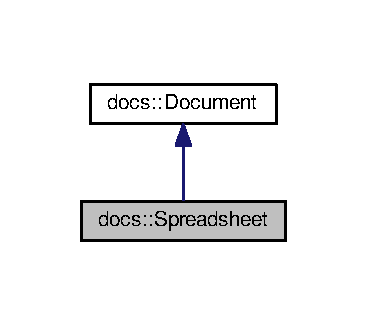
\includegraphics[width=176pt]{classdocs_1_1Spreadsheet__inherit__graph}
\end{center}
\end{figure}


Collaboration diagram for docs\-:\-:Spreadsheet\-:\nopagebreak
\begin{figure}[H]
\begin{center}
\leavevmode
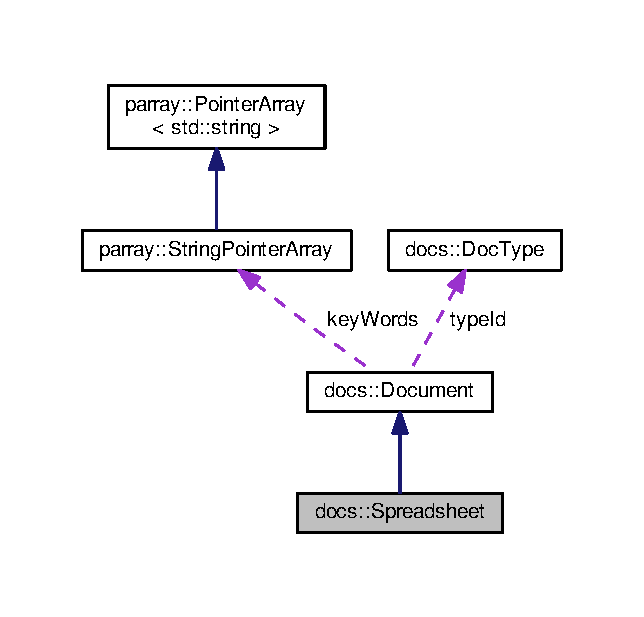
\includegraphics[width=309pt]{classdocs_1_1Spreadsheet__coll__graph}
\end{center}
\end{figure}
\subsection*{Public Member Functions}
\begin{DoxyCompactItemize}
\item 
\hypertarget{classdocs_1_1Spreadsheet_ac6e95d685e342630144afaad04c99c74}{\hyperlink{classdocs_1_1Spreadsheet_ac6e95d685e342630144afaad04c99c74}{Spreadsheet} (int \hyperlink{classdocs_1_1Spreadsheet_a8193931da11e83c62b3aa1c2177e9e33}{coloumn\-Cnt}=\hyperlink{namespacedocs_aa40437dd2d0305c57f338406303a3f58}{D\-E\-F\-A\-U\-L\-T\-\_\-\-S\-P\-R\-E\-A\-D\-S\-H\-E\-E\-T\-\_\-\-C\-O\-L\-C\-N\-T}, int \hyperlink{classdocs_1_1Spreadsheet_a69756007b1fbe6b45d2f052af930d748}{row\-Cnt}=\hyperlink{namespacedocs_a7562daac15433871b1cc71ad74555032}{D\-E\-F\-A\-U\-L\-T\-\_\-\-S\-P\-R\-E\-A\-D\-S\-H\-E\-E\-T\-\_\-\-R\-O\-W\-C\-N\-T}, std\-::string \hyperlink{classdocs_1_1Document_a419e4470c20e1bddd60448ba430f4738}{title}=\hyperlink{namespacedocs_a4cf6dd6732c7e7ab7f7855e440485d89}{D\-E\-F\-A\-U\-L\-T\-\_\-\-D\-O\-C\-U\-M\-E\-N\-T\-\_\-\-T\-I\-T\-L\-E}, int key\-Word\-Size=\hyperlink{namespacedocs_ae635b9481a61628036b5a97625856475}{D\-E\-F\-A\-U\-L\-T\-\_\-\-D\-O\-C\-U\-M\-E\-N\-T\-\_\-\-K\-W\-S\-I\-Z\-E})}\label{classdocs_1_1Spreadsheet_ac6e95d685e342630144afaad04c99c74}

\begin{DoxyCompactList}\small\item\em Construct by creating a new \hyperlink{classdocs_1_1Spreadsheet}{Spreadsheet}. It is based on \hyperlink{classdocs_1_1Document_a9f0b2c4c1a3e3344f374330399969e90}{Document( const Doc\-Type type\-Id, std\-::string, int)} \end{DoxyCompactList}\item 
\hypertarget{classdocs_1_1Spreadsheet_a6dae1de9618f2e4226fde62477858e05}{\hyperlink{classdocs_1_1Spreadsheet_a6dae1de9618f2e4226fde62477858e05}{Spreadsheet} (const \hyperlink{classparray_1_1StringPointerArray}{parray\-::\-String\-Pointer\-Array} \&kws, std\-::string \hyperlink{classdocs_1_1Document_a419e4470c20e1bddd60448ba430f4738}{title}=\hyperlink{namespacedocs_a4cf6dd6732c7e7ab7f7855e440485d89}{D\-E\-F\-A\-U\-L\-T\-\_\-\-D\-O\-C\-U\-M\-E\-N\-T\-\_\-\-T\-I\-T\-L\-E}, int \hyperlink{classdocs_1_1Spreadsheet_a8193931da11e83c62b3aa1c2177e9e33}{coloumn\-Cnt}=\hyperlink{namespacedocs_aa40437dd2d0305c57f338406303a3f58}{D\-E\-F\-A\-U\-L\-T\-\_\-\-S\-P\-R\-E\-A\-D\-S\-H\-E\-E\-T\-\_\-\-C\-O\-L\-C\-N\-T}, int \hyperlink{classdocs_1_1Spreadsheet_a69756007b1fbe6b45d2f052af930d748}{row\-Cnt}=\hyperlink{namespacedocs_a7562daac15433871b1cc71ad74555032}{D\-E\-F\-A\-U\-L\-T\-\_\-\-S\-P\-R\-E\-A\-D\-S\-H\-E\-E\-T\-\_\-\-R\-O\-W\-C\-N\-T})}\label{classdocs_1_1Spreadsheet_a6dae1de9618f2e4226fde62477858e05}

\begin{DoxyCompactList}\small\item\em Construct by creating a new \hyperlink{classdocs_1_1Spreadsheet}{Spreadsheet}. It is based on \hyperlink{classdocs_1_1Document_a4a76d0cee2709582e4b9f3b5b8db0277}{Document( const Doc\-Type type\-Id, const parray\-::\-String\-Pointer\-Array\&, std\-::string title)};. \end{DoxyCompactList}\item 
\hypertarget{classdocs_1_1Spreadsheet_a7bbb06aa9261596202f71c65c5400ff2}{\hyperlink{classdocs_1_1Spreadsheet_a7bbb06aa9261596202f71c65c5400ff2}{Spreadsheet} (const \hyperlink{classdocs_1_1Spreadsheet}{Spreadsheet} \&original)}\label{classdocs_1_1Spreadsheet_a7bbb06aa9261596202f71c65c5400ff2}

\begin{DoxyCompactList}\small\item\em to \hyperlink{classdocs_1_1Spreadsheet_ad7ab608a90b53969ec97214c447c43c6}{copy()} this object \end{DoxyCompactList}\item 
\hypertarget{classdocs_1_1Spreadsheet_a5291016cd2e874e6ce3cf457723fc98c}{virtual \hyperlink{classdocs_1_1Spreadsheet_a5291016cd2e874e6ce3cf457723fc98c}{$\sim$\-Spreadsheet} ()}\label{classdocs_1_1Spreadsheet_a5291016cd2e874e6ce3cf457723fc98c}

\begin{DoxyCompactList}\small\item\em empty destructor,it relies on class hierarchy. \end{DoxyCompactList}\item 
\hypertarget{classdocs_1_1Spreadsheet_ab288d28a2f204e28f0c5d7a097f43bfa}{virtual const std\-::string \hyperlink{classdocs_1_1Spreadsheet_ab288d28a2f204e28f0c5d7a097f43bfa}{to\-String} () const }\label{classdocs_1_1Spreadsheet_ab288d28a2f204e28f0c5d7a097f43bfa}

\begin{DoxyCompactList}\small\item\em append to the result of \hyperlink{classdocs_1_1Document_a16db383045038b779eb489ad125ef02b}{Document\-::to\-String()} the description of the number of columns and rows. \end{DoxyCompactList}\item 
\hypertarget{classdocs_1_1Spreadsheet_a4272d9ebb0edce7d6e3946ca6d08c59b}{virtual const bool \hyperlink{classdocs_1_1Spreadsheet_a4272d9ebb0edce7d6e3946ca6d08c59b}{equals} (const \hyperlink{classdocs_1_1Spreadsheet}{Spreadsheet} \&) const }\label{classdocs_1_1Spreadsheet_a4272d9ebb0edce7d6e3946ca6d08c59b}

\begin{DoxyCompactList}\small\item\em return true if \hyperlink{classdocs_1_1Document_ad86b3a7c7d496f3b05c740e2c1433c78}{Document\-::equals()} is true as well as the number of columns and rows are equals. \end{DoxyCompactList}\item 
\hypertarget{classdocs_1_1Spreadsheet_a25339a2bc1be68500a907969d15b02d0}{const int \hyperlink{classdocs_1_1Spreadsheet_a25339a2bc1be68500a907969d15b02d0}{get\-Row\-Cnt} () const }\label{classdocs_1_1Spreadsheet_a25339a2bc1be68500a907969d15b02d0}

\begin{DoxyCompactList}\small\item\em get the number of rows (\hyperlink{classdocs_1_1Spreadsheet_a69756007b1fbe6b45d2f052af930d748}{row\-Cnt}) of this \hyperlink{classdocs_1_1Spreadsheet}{Spreadsheet}. \end{DoxyCompactList}\item 
\hypertarget{classdocs_1_1Spreadsheet_a2178260b64460a010251eba24513bb9d}{void \hyperlink{classdocs_1_1Spreadsheet_a2178260b64460a010251eba24513bb9d}{set\-Row\-Cnt} (const int)}\label{classdocs_1_1Spreadsheet_a2178260b64460a010251eba24513bb9d}

\begin{DoxyCompactList}\small\item\em set the number of rows (\hyperlink{classdocs_1_1Spreadsheet_a69756007b1fbe6b45d2f052af930d748}{row\-Cnt}) of this \hyperlink{classdocs_1_1Spreadsheet}{Spreadsheet}. \end{DoxyCompactList}\item 
\hypertarget{classdocs_1_1Spreadsheet_a9a89463f0b79318f6ead47bb4d00a7b4}{int \hyperlink{classdocs_1_1Spreadsheet_a9a89463f0b79318f6ead47bb4d00a7b4}{get\-Coloumn\-Cnt} () const }\label{classdocs_1_1Spreadsheet_a9a89463f0b79318f6ead47bb4d00a7b4}

\begin{DoxyCompactList}\small\item\em get the number of columns (\hyperlink{classdocs_1_1Spreadsheet_a8193931da11e83c62b3aa1c2177e9e33}{coloumn\-Cnt}) of this \hyperlink{classdocs_1_1Spreadsheet}{Spreadsheet}. \end{DoxyCompactList}\item 
\hypertarget{classdocs_1_1Spreadsheet_a85e9d8dafdc6793560cb3f1cca41f8e2}{void \hyperlink{classdocs_1_1Spreadsheet_a85e9d8dafdc6793560cb3f1cca41f8e2}{set\-Coloumn\-Cnt} (const int)}\label{classdocs_1_1Spreadsheet_a85e9d8dafdc6793560cb3f1cca41f8e2}

\begin{DoxyCompactList}\small\item\em set the number of columns (\hyperlink{classdocs_1_1Spreadsheet_a8193931da11e83c62b3aa1c2177e9e33}{coloumn\-Cnt}) of this \hyperlink{classdocs_1_1Spreadsheet}{Spreadsheet}. \end{DoxyCompactList}\end{DoxyCompactItemize}
\subsection*{Protected Member Functions}
\begin{DoxyCompactItemize}
\item 
\hypertarget{classdocs_1_1Spreadsheet_ad7ab608a90b53969ec97214c447c43c6}{virtual void \hyperlink{classdocs_1_1Spreadsheet_ad7ab608a90b53969ec97214c447c43c6}{copy} (const \hyperlink{classdocs_1_1Spreadsheet}{Spreadsheet} \&)}\label{classdocs_1_1Spreadsheet_ad7ab608a90b53969ec97214c447c43c6}

\begin{DoxyCompactList}\small\item\em copy this object on a new memory location. It relies on \hyperlink{classdocs_1_1Document_ad8b6a91c7a8e39a880790d14aba14322}{Document\-::copy()}, which is also used on copy constructor and assign operator. \end{DoxyCompactList}\end{DoxyCompactItemize}
\subsection*{Private Attributes}
\begin{DoxyCompactItemize}
\item 
\hypertarget{classdocs_1_1Spreadsheet_a69756007b1fbe6b45d2f052af930d748}{int \hyperlink{classdocs_1_1Spreadsheet_a69756007b1fbe6b45d2f052af930d748}{row\-Cnt}}\label{classdocs_1_1Spreadsheet_a69756007b1fbe6b45d2f052af930d748}

\begin{DoxyCompactList}\small\item\em the number of rows assigned to this \hyperlink{classdocs_1_1Spreadsheet}{Spreadsheet}. \end{DoxyCompactList}\item 
\hypertarget{classdocs_1_1Spreadsheet_a8193931da11e83c62b3aa1c2177e9e33}{int \hyperlink{classdocs_1_1Spreadsheet_a8193931da11e83c62b3aa1c2177e9e33}{coloumn\-Cnt}}\label{classdocs_1_1Spreadsheet_a8193931da11e83c62b3aa1c2177e9e33}

\begin{DoxyCompactList}\small\item\em the number of columns assigned to this \hyperlink{classdocs_1_1Spreadsheet}{Spreadsheet}. \end{DoxyCompactList}\end{DoxyCompactItemize}
\subsection*{Additional Inherited Members}


\subsection{Detailed Description}
This describes a \hyperlink{classdocs_1_1Document}{Document} which has also a specified number of columns and rows. 

The documentation for this class was generated from the following files\-:\begin{DoxyCompactItemize}
\item 
src/\hyperlink{Document_8h}{Document.\-h}\item 
src/\hyperlink{Spreadsheet_8cpp}{Spreadsheet.\-cpp}\end{DoxyCompactItemize}

\hypertarget{classparray_1_1StringPointerArray}{\section{parray\-:\-:String\-Pointer\-Array Class Reference}
\label{classparray_1_1StringPointerArray}\index{parray\-::\-String\-Pointer\-Array@{parray\-::\-String\-Pointer\-Array}}
}


Inheritance diagram for parray\-:\-:String\-Pointer\-Array\-:\nopagebreak
\begin{figure}[H]
\begin{center}
\leavevmode
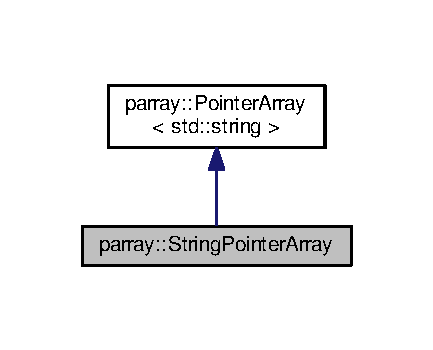
\includegraphics[width=208pt]{classparray_1_1StringPointerArray__inherit__graph}
\end{center}
\end{figure}


Collaboration diagram for parray\-:\-:String\-Pointer\-Array\-:\nopagebreak
\begin{figure}[H]
\begin{center}
\leavevmode
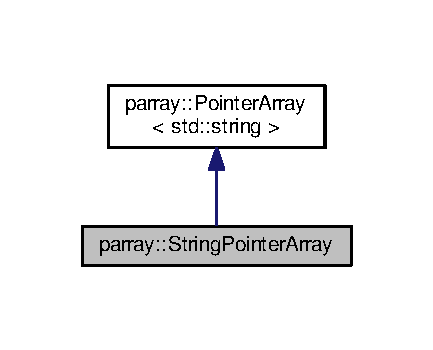
\includegraphics[width=208pt]{classparray_1_1StringPointerArray__coll__graph}
\end{center}
\end{figure}
\subsection*{Public Member Functions}
\begin{DoxyCompactItemize}
\item 
\hypertarget{classparray_1_1StringPointerArray_a3dcc569f7833b31b26bb72570bdc7067}{\hyperlink{classparray_1_1StringPointerArray_a3dcc569f7833b31b26bb72570bdc7067}{String\-Pointer\-Array} ()}\label{classparray_1_1StringPointerArray_a3dcc569f7833b31b26bb72570bdc7067}

\begin{DoxyCompactList}\small\item\em empty constructor, based on \hyperlink{classparray_1_1PointerArray_ab506b284822d1e013813579e06893797}{Pointer\-Array\-::\-Pointer\-Array()}. \end{DoxyCompactList}\item 
\hypertarget{classparray_1_1StringPointerArray_ae31ac6c33c13c602d3cbee3ca4aed10c}{\hyperlink{classparray_1_1StringPointerArray_ae31ac6c33c13c602d3cbee3ca4aed10c}{String\-Pointer\-Array} (const int length)}\label{classparray_1_1StringPointerArray_ae31ac6c33c13c602d3cbee3ca4aed10c}

\begin{DoxyCompactList}\small\item\em constructor a new array of given length, based on \hyperlink{classparray_1_1PointerArray_a4e39d7adf15e94c02dfe2662c181f0c6}{Pointer\-Array\-::\-Pointer\-Array( int)}. \end{DoxyCompactList}\item 
\hypertarget{classparray_1_1StringPointerArray_a6566d7032d0c519b440220df77651345}{\hyperlink{classparray_1_1StringPointerArray_a6566d7032d0c519b440220df77651345}{String\-Pointer\-Array} (const \hyperlink{classparray_1_1StringPointerArray}{String\-Pointer\-Array} \&original)}\label{classparray_1_1StringPointerArray_a6566d7032d0c519b440220df77651345}

\begin{DoxyCompactList}\small\item\em \hyperlink{classparray_1_1PointerArray_a3010540e156076377ffd4428b05e1ac2}{Pointer\-Array\-::copy()} constructor, based on Pointer\-Array\-::\-Pointer\-Array( Pointer\-Array). \end{DoxyCompactList}\item 
\hypertarget{classparray_1_1StringPointerArray_a66e413fa7aedbfe9b45c87d8641ea36e}{virtual \hyperlink{classparray_1_1StringPointerArray_a66e413fa7aedbfe9b45c87d8641ea36e}{$\sim$\-String\-Pointer\-Array} ()}\label{classparray_1_1StringPointerArray_a66e413fa7aedbfe9b45c87d8641ea36e}

\begin{DoxyCompactList}\small\item\em empty destructor, it relies on the base implementation. \end{DoxyCompactList}\item 
\hypertarget{classparray_1_1StringPointerArray_a5b79fa79d5aa75cd4572e7b87f6da25f}{virtual bool \hyperlink{classparray_1_1StringPointerArray_a5b79fa79d5aa75cd4572e7b87f6da25f}{add} (std\-::string to\-Add)}\label{classparray_1_1StringPointerArray_a5b79fa79d5aa75cd4572e7b87f6da25f}

\begin{DoxyCompactList}\small\item\em overload the \hyperlink{classparray_1_1PointerArray_ae080aeced3af072006e4a609fdadb838}{Pointer\-Array\-::add()} method by call \hyperlink{classparray_1_1PointerArray_a6d4347a899d2783d23775957ad71f743}{resize} if the array is full (generate warning). \end{DoxyCompactList}\end{DoxyCompactItemize}
\subsection*{Static Public Member Functions}
\begin{DoxyCompactItemize}
\item 
static void \hyperlink{classparray_1_1StringPointerArray_abfac13570bec8c88311714d19ddea59b}{tester} ()
\begin{DoxyCompactList}\small\item\em static method to test the behavior of a \hyperlink{classparray_1_1PointerArray}{Pointer\-Array} of strings. \end{DoxyCompactList}\end{DoxyCompactItemize}
\subsection*{Static Private Member Functions}
\begin{DoxyCompactItemize}
\item 
\hypertarget{classparray_1_1StringPointerArray_a17703cd98a2019970fccba1bc7e51c8e}{static void \hyperlink{classparray_1_1StringPointerArray_a17703cd98a2019970fccba1bc7e51c8e}{print\-Test\-Delitator} ()}\label{classparray_1_1StringPointerArray_a17703cd98a2019970fccba1bc7e51c8e}

\begin{DoxyCompactList}\small\item\em prints a line to separe different tests used in \hyperlink{classparray_1_1StringPointerArray_abfac13570bec8c88311714d19ddea59b}{tester()} function \end{DoxyCompactList}\end{DoxyCompactItemize}


\subsection{Detailed Description}
It implements a dynamic array of (T=)string manager. \begin{DoxySeeAlso}{See Also}
\hyperlink{classparray_1_1PointerArray}{Pointer\-Array} 
\end{DoxySeeAlso}


\subsection{Member Function Documentation}
\hypertarget{classparray_1_1StringPointerArray_abfac13570bec8c88311714d19ddea59b}{\index{parray\-::\-String\-Pointer\-Array@{parray\-::\-String\-Pointer\-Array}!tester@{tester}}
\index{tester@{tester}!parray::StringPointerArray@{parray\-::\-String\-Pointer\-Array}}
\subsubsection[{tester}]{\setlength{\rightskip}{0pt plus 5cm}static void parray\-::\-String\-Pointer\-Array\-::tester (
\begin{DoxyParamCaption}
{}
\end{DoxyParamCaption}
)\hspace{0.3cm}{\ttfamily [inline]}, {\ttfamily [static]}}}\label{classparray_1_1StringPointerArray_abfac13570bec8c88311714d19ddea59b}


static method to test the behavior of a \hyperlink{classparray_1_1PointerArray}{Pointer\-Array} of strings. 

Creates (pa0) new parray\-::\-String\-Point\-Array( const int) and populate with letters.

String\-Pointer\-Array\-::remove( T) an element from pa0 and access the first char (\hyperlink{classparray_1_1PointerArray_aa009614c6819fe08b7eef78be4394dbc}{String\-Pointer\-Array\-::operator\mbox{[}$\,$\mbox{]}()}) after the manipulation.

Creates (pa1) a new \#\-String\-Point\-Array() and set is size to be smaller than pa0.

Populate (\hyperlink{classparray_1_1StringPointerArray_a5b79fa79d5aa75cd4572e7b87f6da25f}{String\-Pointer\-Array\-::add()}) pa1 with some elements.

Make a comparison (\hyperlink{classparray_1_1PointerArray_a050d55aeebf51f02bf59d8352664528d}{String\-Pointer\-Array\-::operator==()}) between two \hyperlink{classparray_1_1StringPointerArray_a3dcc569f7833b31b26bb72570bdc7067}{String\-Pointer\-Array} (pa0 == pa1)

Creates (pa2) a copy (\hyperlink{classparray_1_1PointerArray_a3010540e156076377ffd4428b05e1ac2}{String\-Pointer\-Array\-::copy()} and String\-Pointer\-Array(\-String\-Pointer\-Array)) of pa1.

\hyperlink{classparray_1_1PointerArray_a13ae3b9b2118416351cc63bd456ecf73}{String\-Pointer\-Array\-::remove()} all its elements and makes a comparison.

Adds two strings to pa2.

Creates (pa3) a \hyperlink{classparray_1_1PointerArray_a3010540e156076377ffd4428b05e1ac2}{copy()} of pa2 and remove the first element.

Makes a comparison (pa3 == pa2) and \hyperlink{classparray_1_1PointerArray_a13883fc7ef994a50a83ae3f9ddc4db27}{pack()} pa2.

\hyperlink{classparray_1_1PointerArray_a6d4347a899d2783d23775957ad71f743}{resize()} pa1 to be bigger and smaller. 

Here is the call graph for this function\-:\nopagebreak
\begin{figure}[H]
\begin{center}
\leavevmode
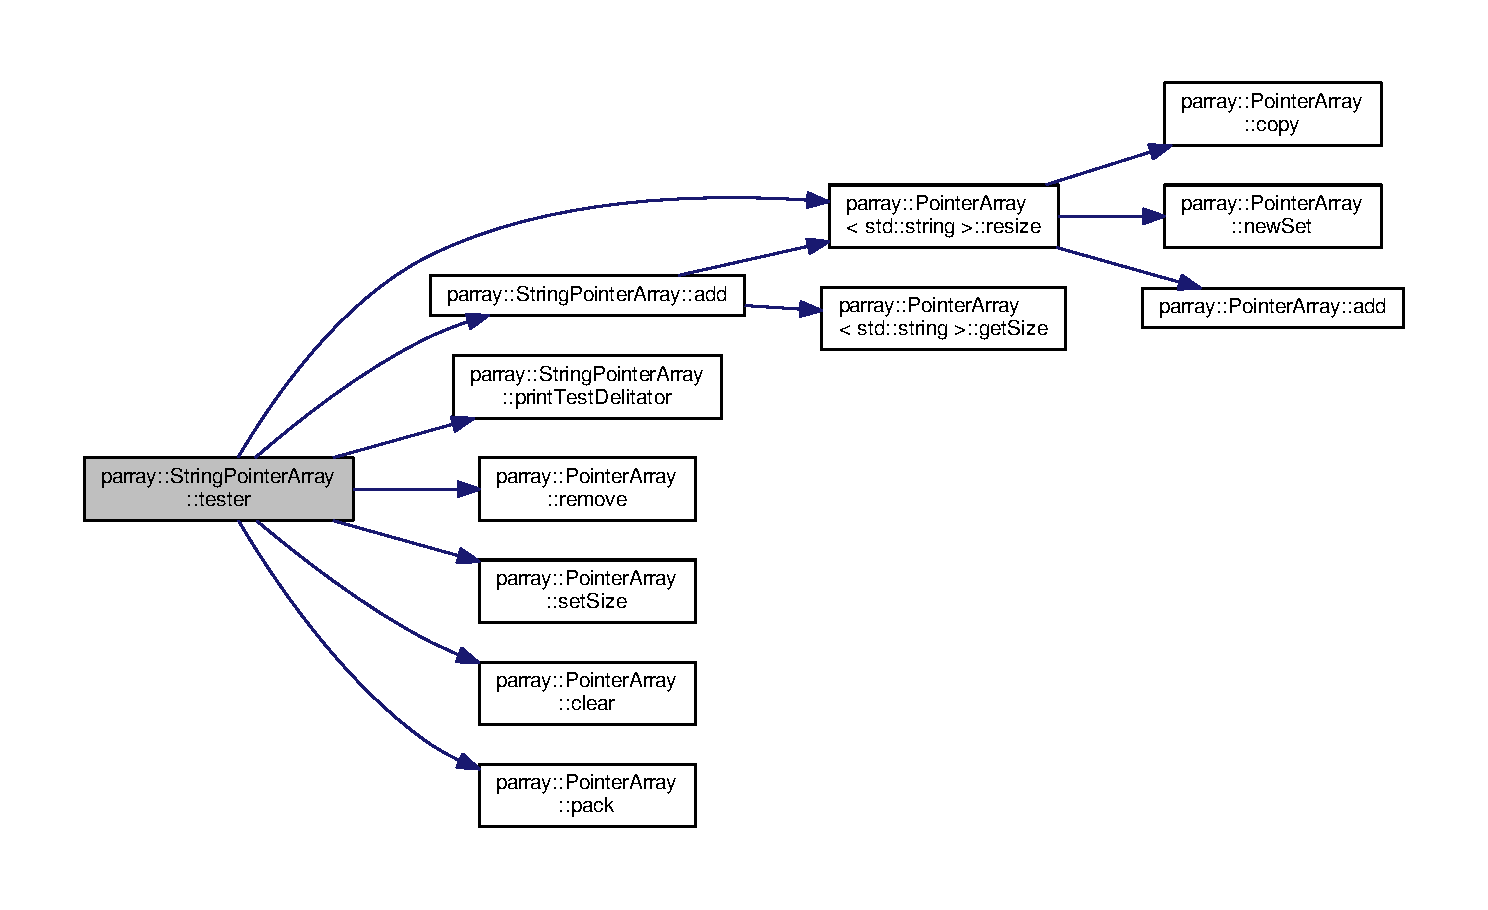
\includegraphics[width=350pt]{classparray_1_1StringPointerArray_abfac13570bec8c88311714d19ddea59b_cgraph}
\end{center}
\end{figure}




The documentation for this class was generated from the following file\-:\begin{DoxyCompactItemize}
\item 
src/\hyperlink{PointerArray_8cpp}{Pointer\-Array.\-cpp}\end{DoxyCompactItemize}

\hypertarget{classdocs_1_1WebPage}{\section{docs\-:\-:Web\-Page Class Reference}
\label{classdocs_1_1WebPage}\index{docs\-::\-Web\-Page@{docs\-::\-Web\-Page}}
}


{\ttfamily \#include $<$Document.\-h$>$}



Inheritance diagram for docs\-:\-:Web\-Page\-:\nopagebreak
\begin{figure}[H]
\begin{center}
\leavevmode
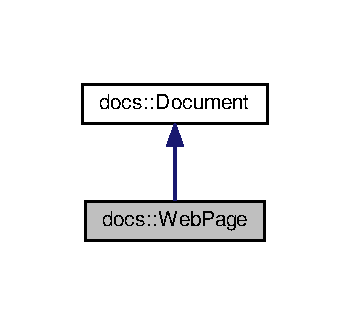
\includegraphics[width=168pt]{classdocs_1_1WebPage__inherit__graph}
\end{center}
\end{figure}


Collaboration diagram for docs\-:\-:Web\-Page\-:\nopagebreak
\begin{figure}[H]
\begin{center}
\leavevmode
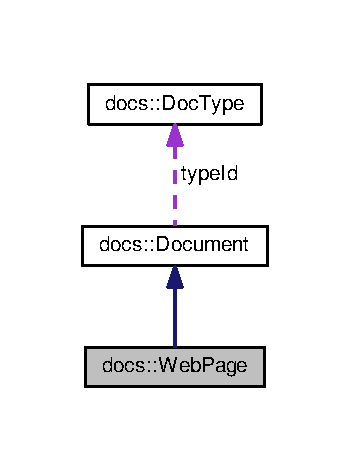
\includegraphics[width=309pt]{classdocs_1_1WebPage__coll__graph}
\end{center}
\end{figure}
\subsection*{Public Member Functions}
\begin{DoxyCompactItemize}
\item 
\hypertarget{classdocs_1_1WebPage_a9642db10cbcecf7fd93338f936318e90}{\hyperlink{classdocs_1_1WebPage_a9642db10cbcecf7fd93338f936318e90}{Web\-Page} (std\-::string \hyperlink{classdocs_1_1Document_a419e4470c20e1bddd60448ba430f4738}{title}=\hyperlink{namespacedocs_a4cf6dd6732c7e7ab7f7855e440485d89}{D\-E\-F\-A\-U\-L\-T\-\_\-\-D\-O\-C\-U\-M\-E\-N\-T\-\_\-\-T\-I\-T\-L\-E}, std\-::string \hyperlink{classdocs_1_1WebPage_a4495e463a26d77b22ec4d8af690bbb11}{url}=\hyperlink{namespacedocs_a9bfb062436ca30729256c522cf54c111}{D\-E\-F\-A\-U\-L\-T\-\_\-\-W\-E\-B\-P\-A\-G\-E\-\_\-\-U\-R\-L}, int key\-Word\-Size=\hyperlink{namespacedocs_ae635b9481a61628036b5a97625856475}{D\-E\-F\-A\-U\-L\-T\-\_\-\-D\-O\-C\-U\-M\-E\-N\-T\-\_\-\-K\-W\-S\-I\-Z\-E}, int text\-Size=\hyperlink{namespacedocs_a966b8c0a825e3e04a2c667abefa97f41}{D\-E\-F\-A\-U\-L\-T\-\_\-\-W\-E\-B\-P\-A\-G\-E\-\_\-\-T\-E\-X\-T\-S\-I\-Z\-E})}\label{classdocs_1_1WebPage_a9642db10cbcecf7fd93338f936318e90}

\begin{DoxyCompactList}\small\item\em construct by creating a new contents list. It is based on \hyperlink{classdocs_1_1Document_a9f0b2c4c1a3e3344f374330399969e90}{Document( const Doc\-Type type\-Id, std\-::string, int)} \end{DoxyCompactList}\item 
\hypertarget{classdocs_1_1WebPage_a7013883a569946e65ba6522c878b0517}{\hyperlink{classdocs_1_1WebPage_a7013883a569946e65ba6522c878b0517}{Web\-Page} (const \hyperlink{classparray_1_1StringPointerArray}{parray\-::\-String\-Pointer\-Array} \&kws, const \hyperlink{classparray_1_1StringPointerArray}{parray\-::\-String\-Pointer\-Array} \&tex=0, std\-::string \hyperlink{classdocs_1_1Document_a419e4470c20e1bddd60448ba430f4738}{title}=\hyperlink{namespacedocs_a4cf6dd6732c7e7ab7f7855e440485d89}{D\-E\-F\-A\-U\-L\-T\-\_\-\-D\-O\-C\-U\-M\-E\-N\-T\-\_\-\-T\-I\-T\-L\-E}, std\-::string \hyperlink{classdocs_1_1WebPage_a4495e463a26d77b22ec4d8af690bbb11}{url}=\hyperlink{namespacedocs_a9bfb062436ca30729256c522cf54c111}{D\-E\-F\-A\-U\-L\-T\-\_\-\-W\-E\-B\-P\-A\-G\-E\-\_\-\-U\-R\-L})}\label{classdocs_1_1WebPage_a7013883a569946e65ba6522c878b0517}

\begin{DoxyCompactList}\small\item\em construct by using a copy of a Pointer\-Array of contents. It is based on \hyperlink{classdocs_1_1Document_a4a76d0cee2709582e4b9f3b5b8db0277}{Document( const Doc\-Type type\-Id, const parray\-::\-String\-Pointer\-Array\&, std\-::string title)}; \end{DoxyCompactList}\item 
\hypertarget{classdocs_1_1WebPage_a4c2ea40e27d1763d3f7c2c5055518a41}{\hyperlink{classdocs_1_1WebPage_a4c2ea40e27d1763d3f7c2c5055518a41}{Web\-Page} (const \hyperlink{classdocs_1_1WebPage}{Web\-Page} \&original)}\label{classdocs_1_1WebPage_a4c2ea40e27d1763d3f7c2c5055518a41}

\begin{DoxyCompactList}\small\item\em to \hyperlink{classdocs_1_1WebPage_a52ac0dc90ab3f5621d0fa41d8386806c}{copy()} this object \end{DoxyCompactList}\item 
\hypertarget{classdocs_1_1WebPage_a20af4ea1f7d488ae695b316a604ea6ad}{virtual \hyperlink{classdocs_1_1WebPage_a20af4ea1f7d488ae695b316a604ea6ad}{$\sim$\-Web\-Page} ()}\label{classdocs_1_1WebPage_a20af4ea1f7d488ae695b316a604ea6ad}

\begin{DoxyCompactList}\small\item\em destructor, to clear the contents list. \end{DoxyCompactList}\item 
\hypertarget{classdocs_1_1WebPage_ac3d747b84fa4e357791faab5994ccc22}{virtual const std\-::string \hyperlink{classdocs_1_1WebPage_ac3d747b84fa4e357791faab5994ccc22}{to\-String} () const }\label{classdocs_1_1WebPage_ac3d747b84fa4e357791faab5994ccc22}

\begin{DoxyCompactList}\small\item\em append to the result of \hyperlink{classdocs_1_1Document_a16db383045038b779eb489ad125ef02b}{Document\-::to\-String()} the description of the url and contents. \end{DoxyCompactList}\item 
\hypertarget{classdocs_1_1WebPage_aaced244fd624030e82026ba294282615}{virtual const bool \hyperlink{classdocs_1_1WebPage_aaced244fd624030e82026ba294282615}{equals} (const \hyperlink{classdocs_1_1WebPage}{Web\-Page} \&) const }\label{classdocs_1_1WebPage_aaced244fd624030e82026ba294282615}

\begin{DoxyCompactList}\small\item\em return true if \hyperlink{classdocs_1_1Document_ad86b3a7c7d496f3b05c740e2c1433c78}{Document\-::equals()} is true as well as urls and contends are equals. \end{DoxyCompactList}\item 
\hypertarget{classdocs_1_1WebPage_aaeac2076cad36b3dd2c3ea090e4712e0}{virtual const std\-::string \hyperlink{classdocs_1_1WebPage_aaeac2076cad36b3dd2c3ea090e4712e0}{get\-Url} () const }\label{classdocs_1_1WebPage_aaeac2076cad36b3dd2c3ea090e4712e0}

\begin{DoxyCompactList}\small\item\em returns the \hyperlink{classdocs_1_1WebPage_a4495e463a26d77b22ec4d8af690bbb11}{url} assign to this web page. \end{DoxyCompactList}\item 
\hypertarget{classdocs_1_1WebPage_a46ae47ff938c8b9a4081c17b2c307ef9}{virtual void \hyperlink{classdocs_1_1WebPage_a46ae47ff938c8b9a4081c17b2c307ef9}{set\-Url} (const std\-::string)}\label{classdocs_1_1WebPage_a46ae47ff938c8b9a4081c17b2c307ef9}

\begin{DoxyCompactList}\small\item\em set the \hyperlink{classdocs_1_1WebPage_a4495e463a26d77b22ec4d8af690bbb11}{url} for this web page \end{DoxyCompactList}\item 
\hypertarget{classdocs_1_1WebPage_ad2efbd306365a023f52c5c93caa4e638}{virtual \\*
\hyperlink{classparray_1_1StringPointerArray}{parray\-::\-String\-Pointer\-Array} $\ast$ \hyperlink{classdocs_1_1WebPage_ad2efbd306365a023f52c5c93caa4e638}{get\-Contents} () const }\label{classdocs_1_1WebPage_ad2efbd306365a023f52c5c93caa4e638}

\begin{DoxyCompactList}\small\item\em returns the manager of the \hyperlink{classdocs_1_1WebPage_a67d46a145ff4e7093fb1b8f56e539895}{contents} array of this document. \end{DoxyCompactList}\item 
\hypertarget{classdocs_1_1WebPage_a2e09e939689a61083a5037dcc7f84419}{virtual void \hyperlink{classdocs_1_1WebPage_a2e09e939689a61083a5037dcc7f84419}{set\-Contents} (\hyperlink{classparray_1_1StringPointerArray}{parray\-::\-String\-Pointer\-Array} $\ast$)}\label{classdocs_1_1WebPage_a2e09e939689a61083a5037dcc7f84419}

\begin{DoxyCompactList}\small\item\em set a copy of the input \hyperlink{classdocs_1_1WebPage_a67d46a145ff4e7093fb1b8f56e539895}{contents} and overwrites the previous. \end{DoxyCompactList}\item 
\hypertarget{classdocs_1_1WebPage_a7bebbf9d6f6ed1d5d37807ce14a34b2b}{virtual const std\-::string $\ast$ \hyperlink{classdocs_1_1WebPage_a7bebbf9d6f6ed1d5d37807ce14a34b2b}{get\-Contents\-Array} () const }\label{classdocs_1_1WebPage_a7bebbf9d6f6ed1d5d37807ce14a34b2b}

\begin{DoxyCompactList}\small\item\em returns the dynamic array containing the \hyperlink{classdocs_1_1WebPage_a67d46a145ff4e7093fb1b8f56e539895}{contents}. \end{DoxyCompactList}\item 
\hypertarget{classdocs_1_1WebPage_ae58ebf97dc7208acbd7b86b267f3b699}{virtual const int \hyperlink{classdocs_1_1WebPage_ae58ebf97dc7208acbd7b86b267f3b699}{get\-Contents\-Size} () const }\label{classdocs_1_1WebPage_ae58ebf97dc7208acbd7b86b267f3b699}

\begin{DoxyCompactList}\small\item\em returns the \hyperlink{classdocs_1_1WebPage_a7bebbf9d6f6ed1d5d37807ce14a34b2b}{get\-Contents\-Array()} size \end{DoxyCompactList}\end{DoxyCompactItemize}
\subsection*{Protected Member Functions}
\begin{DoxyCompactItemize}
\item 
\hypertarget{classdocs_1_1WebPage_a52ac0dc90ab3f5621d0fa41d8386806c}{virtual void \hyperlink{classdocs_1_1WebPage_a52ac0dc90ab3f5621d0fa41d8386806c}{copy} (const \hyperlink{classdocs_1_1WebPage}{Web\-Page} \&)}\label{classdocs_1_1WebPage_a52ac0dc90ab3f5621d0fa41d8386806c}

\begin{DoxyCompactList}\small\item\em copy this object on a new memory location. It relies on \hyperlink{classdocs_1_1Document_ad8b6a91c7a8e39a880790d14aba14322}{Document\-::copy()}, which is also used on copy constructor and assign operator. \end{DoxyCompactList}\end{DoxyCompactItemize}
\subsection*{Private Attributes}
\begin{DoxyCompactItemize}
\item 
\hypertarget{classdocs_1_1WebPage_a4495e463a26d77b22ec4d8af690bbb11}{std\-::string \hyperlink{classdocs_1_1WebPage_a4495e463a26d77b22ec4d8af690bbb11}{url}}\label{classdocs_1_1WebPage_a4495e463a26d77b22ec4d8af690bbb11}

\begin{DoxyCompactList}\small\item\em The url of this \hyperlink{classdocs_1_1WebPage}{Web\-Page}. \end{DoxyCompactList}\item 
\hypertarget{classdocs_1_1WebPage_a67d46a145ff4e7093fb1b8f56e539895}{\hyperlink{classparray_1_1StringPointerArray}{parray\-::\-String\-Pointer\-Array} $\ast$ \hyperlink{classdocs_1_1WebPage_a67d46a145ff4e7093fb1b8f56e539895}{contents}}\label{classdocs_1_1WebPage_a67d46a145ff4e7093fb1b8f56e539895}

\begin{DoxyCompactList}\small\item\em The contents of this \hyperlink{classdocs_1_1WebPage}{Web\-Page}. \end{DoxyCompactList}\end{DoxyCompactItemize}
\subsection*{Additional Inherited Members}


\subsection{Detailed Description}
It describes a web page as a \hyperlink{classdocs_1_1Document}{Document} which have also an url and an array of contents (e.\-g., textual line). 

The documentation for this class was generated from the following files\-:\begin{DoxyCompactItemize}
\item 
src/\hyperlink{Document_8h}{Document.\-h}\item 
src/\hyperlink{WebPage_8cpp}{Web\-Page.\-cpp}\end{DoxyCompactItemize}

\chapter{File Documentation}
\hypertarget{Document_8cpp}{\section{src/\-Document.cpp File Reference}
\label{Document_8cpp}\index{src/\-Document.\-cpp@{src/\-Document.\-cpp}}
}


implementation of the Document base class.  


{\ttfamily \#include \char`\"{}Document.\-h\char`\"{}}\\*
Include dependency graph for Document.\-cpp\-:\nopagebreak
\begin{figure}[H]
\begin{center}
\leavevmode
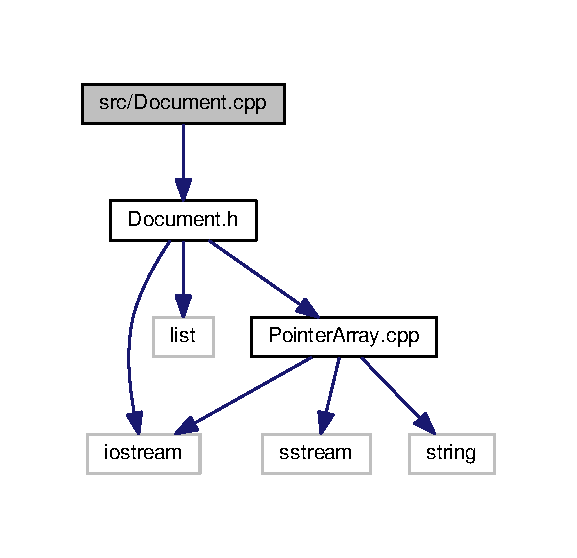
\includegraphics[width=277pt]{Document_8cpp__incl}
\end{center}
\end{figure}
\subsection*{Namespaces}
\begin{DoxyCompactItemize}
\item 
\hyperlink{namespacedocs}{docs}
\begin{DoxyCompactList}\small\item\em This namespace is used to collect all the document hierarchy classes and types. \end{DoxyCompactList}\end{DoxyCompactItemize}
\subsection*{Functions}
\begin{DoxyCompactItemize}
\item 
std\-::ostream \& \hyperlink{namespacedocs_a2464f4b0ad981aa2f4f4f56dd16afb18}{docs\-::operator$<$$<$} (std\-::ostream \&strm, const Document \&doc)
\item 
bool \hyperlink{namespacedocs_a69ecd221cb71a7f629bf48b283aefbc2}{docs\-::operator==} (const Document \&c1, const Document \&c2)
\item 
bool \hyperlink{namespacedocs_abbb9bd3baf3e28ceb50a275bb0695e89}{docs\-::operator!=} (const Document \&c1, const Document \&c2)
\end{DoxyCompactItemize}


\subsection{Detailed Description}
implementation of the Document base class. \begin{DoxyAuthor}{Author}
Buoncompagni Luca 
\end{DoxyAuthor}
\begin{DoxyDate}{Date}
Sep 14, 2016
\end{DoxyDate}
\begin{DoxySeeAlso}{See Also}
Document 

\hyperlink{namespacedocs}{docs} 
\end{DoxySeeAlso}


Definition in file \hyperlink{Document_8cpp_source}{Document.\-cpp}.


\hypertarget{Document_8h}{\section{src/\-Document.h File Reference}
\label{Document_8h}\index{src/\-Document.\-h@{src/\-Document.\-h}}
}


The complete Document Hierarchy namespce specification.  


{\ttfamily \#include $<$iostream$>$}\\*
{\ttfamily \#include $<$list$>$}\\*
{\ttfamily \#include \char`\"{}Pointer\-Array.\-cpp\char`\"{}}\\*
Include dependency graph for Document.\-h\-:\nopagebreak
\begin{figure}[H]
\begin{center}
\leavevmode
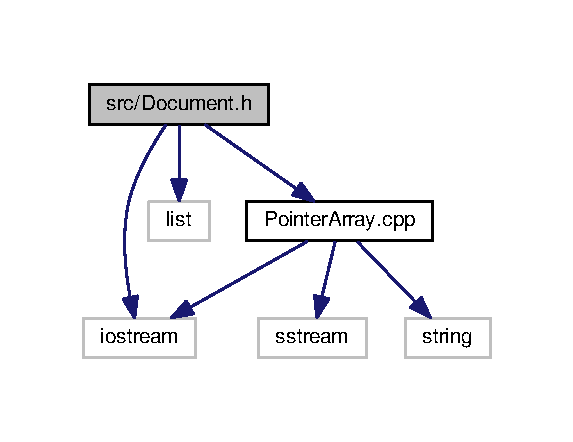
\includegraphics[width=275pt]{Document_8h__incl}
\end{center}
\end{figure}
This graph shows which files directly or indirectly include this file\-:\nopagebreak
\begin{figure}[H]
\begin{center}
\leavevmode
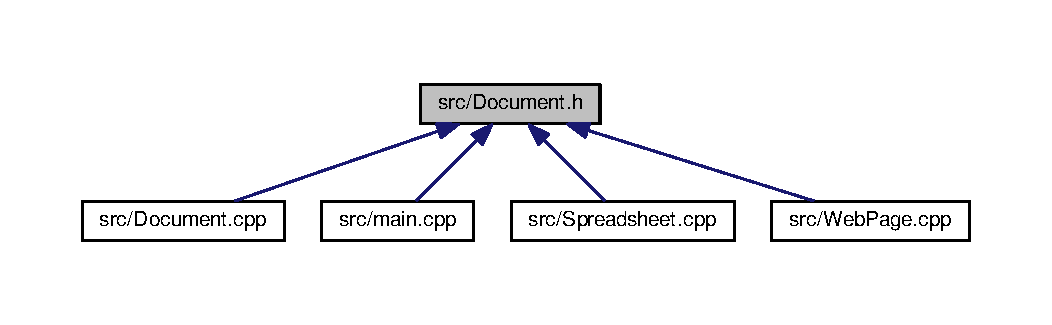
\includegraphics[width=350pt]{Document_8h__dep__incl}
\end{center}
\end{figure}
\subsection*{Classes}
\begin{DoxyCompactItemize}
\item 
class \hyperlink{classdocs_1_1DocType}{docs\-::\-Doc\-Type}
\begin{DoxyCompactList}\small\item\em The class containing the definition of \hyperlink{classdocs_1_1Document}{Document} Types names. \end{DoxyCompactList}\item 
class \hyperlink{classdocs_1_1Document}{docs\-::\-Document}
\begin{DoxyCompactList}\small\item\em This is the base class of the \hyperlink{classdocs_1_1Document}{Document} hierarchy. \end{DoxyCompactList}\item 
class \hyperlink{classdocs_1_1WebPage}{docs\-::\-Web\-Page}
\begin{DoxyCompactList}\small\item\em It describes a web page as a \hyperlink{classdocs_1_1Document}{Document} extensions. \end{DoxyCompactList}\item 
class \hyperlink{classdocs_1_1Spreadsheet}{docs\-::\-Spreadsheet}
\begin{DoxyCompactList}\small\item\em This describes a spreadsheet as a \hyperlink{classdocs_1_1Document}{Document} extension. \end{DoxyCompactList}\end{DoxyCompactItemize}
\subsection*{Namespaces}
\begin{DoxyCompactItemize}
\item 
\hyperlink{namespacedocs}{docs}
\begin{DoxyCompactList}\small\item\em This namespace is used to collect all the document hierarchy classes and types. \end{DoxyCompactList}\end{DoxyCompactItemize}
\subsection*{Enumerations}
\begin{DoxyCompactItemize}
\item 
enum \hyperlink{namespacedocs_a150efca62822b8ab62a5afabe299bf75}{docs\-::\-Type} \{ \hyperlink{namespacedocs_a150efca62822b8ab62a5afabe299bf75ab5b85a2de45c75c8eb58ccb377a01543}{docs\-::\-D\-O\-C\-U\-M\-E\-N\-T}, 
\hyperlink{namespacedocs_a150efca62822b8ab62a5afabe299bf75a1660685efab992a33bb802d68b4e8c13}{docs\-::\-W\-E\-B\-\_\-\-P\-A\-G\-E}, 
\hyperlink{namespacedocs_a150efca62822b8ab62a5afabe299bf75a7c469773c8012b650a4db4d9f46e343a}{docs\-::\-S\-P\-R\-E\-A\-D\-S\-H\-E\-E\-T}
 \}
\begin{DoxyCompactList}\small\item\em Instances of document identifier values. \end{DoxyCompactList}\end{DoxyCompactItemize}
\subsection*{Variables}
\begin{DoxyCompactItemize}
\item 
\hypertarget{namespacedocs_a4cf6dd6732c7e7ab7f7855e440485d89}{const std\-::string \hyperlink{namespacedocs_a4cf6dd6732c7e7ab7f7855e440485d89}{docs\-::\-D\-E\-F\-A\-U\-L\-T\-\_\-\-D\-O\-C\-U\-M\-E\-N\-T\-\_\-\-T\-I\-T\-L\-E} = \char`\"{}Default Title\char`\"{}}\label{namespacedocs_a4cf6dd6732c7e7ab7f7855e440485d89}

\begin{DoxyCompactList}\small\item\em The title, if not specified on \hyperlink{classdocs_1_1Document}{Document} construction. \end{DoxyCompactList}\item 
\hypertarget{namespacedocs_ae635b9481a61628036b5a97625856475}{const int \hyperlink{namespacedocs_ae635b9481a61628036b5a97625856475}{docs\-::\-D\-E\-F\-A\-U\-L\-T\-\_\-\-D\-O\-C\-U\-M\-E\-N\-T\-\_\-\-K\-W\-S\-I\-Z\-E} = 3}\label{namespacedocs_ae635b9481a61628036b5a97625856475}

\begin{DoxyCompactList}\small\item\em The size, of key words if not specified on \hyperlink{classdocs_1_1Document}{Document} construction. \end{DoxyCompactList}\item 
\hypertarget{namespacedocs_a9bfb062436ca30729256c522cf54c111}{const std\-::string \hyperlink{namespacedocs_a9bfb062436ca30729256c522cf54c111}{docs\-::\-D\-E\-F\-A\-U\-L\-T\-\_\-\-W\-E\-B\-P\-A\-G\-E\-\_\-\-U\-R\-L} = \char`\"{}www.\-defualt.\-com\char`\"{}}\label{namespacedocs_a9bfb062436ca30729256c522cf54c111}

\begin{DoxyCompactList}\small\item\em The url, if not specified on \hyperlink{classdocs_1_1WebPage}{Web\-Page} construction. \end{DoxyCompactList}\item 
\hypertarget{namespacedocs_a966b8c0a825e3e04a2c667abefa97f41}{const int \hyperlink{namespacedocs_a966b8c0a825e3e04a2c667abefa97f41}{docs\-::\-D\-E\-F\-A\-U\-L\-T\-\_\-\-W\-E\-B\-P\-A\-G\-E\-\_\-\-T\-E\-X\-T\-S\-I\-Z\-E} = 10}\label{namespacedocs_a966b8c0a825e3e04a2c667abefa97f41}

\begin{DoxyCompactList}\small\item\em The size of contents, if not specified on \hyperlink{classdocs_1_1WebPage}{Web\-Page} construction. \end{DoxyCompactList}\item 
\hypertarget{namespacedocs_aa40437dd2d0305c57f338406303a3f58}{const int \hyperlink{namespacedocs_aa40437dd2d0305c57f338406303a3f58}{docs\-::\-D\-E\-F\-A\-U\-L\-T\-\_\-\-S\-P\-R\-E\-A\-D\-S\-H\-E\-E\-T\-\_\-\-C\-O\-L\-C\-N\-T} = 7}\label{namespacedocs_aa40437dd2d0305c57f338406303a3f58}

\begin{DoxyCompactList}\small\item\em The number of columns, if not specified on \hyperlink{classdocs_1_1Spreadsheet}{Spreadsheet} construction. \end{DoxyCompactList}\item 
\hypertarget{namespacedocs_a7562daac15433871b1cc71ad74555032}{const int \hyperlink{namespacedocs_a7562daac15433871b1cc71ad74555032}{docs\-::\-D\-E\-F\-A\-U\-L\-T\-\_\-\-S\-P\-R\-E\-A\-D\-S\-H\-E\-E\-T\-\_\-\-R\-O\-W\-C\-N\-T} = 2}\label{namespacedocs_a7562daac15433871b1cc71ad74555032}

\begin{DoxyCompactList}\small\item\em The number of rows, if not specified on \hyperlink{classdocs_1_1Spreadsheet}{Spreadsheet} construction. \end{DoxyCompactList}\item 
\hypertarget{namespacedocs_a88f8e41b03147cf4197261676999d12c}{const std\-::string \hyperlink{namespacedocs_a88f8e41b03147cf4197261676999d12c}{docs\-::\-T\-Y\-P\-E\-\_\-\-N\-A\-M\-E\-\_\-\-D\-O\-C\-U\-M\-E\-N\-T} = \char`\"{}\textbackslash{}\char`\"{}Document\textbackslash{}\char`\"{}\char`\"{}}\label{namespacedocs_a88f8e41b03147cf4197261676999d12c}

\begin{DoxyCompactList}\small\item\em The name of the Type.\-D\-O\-C\-U\-M\-E\-N\-T type values. \end{DoxyCompactList}\item 
\hypertarget{namespacedocs_ac41cf3635e22c3750deddd000fd4c34b}{const std\-::string \hyperlink{namespacedocs_ac41cf3635e22c3750deddd000fd4c34b}{docs\-::\-T\-Y\-P\-E\-\_\-\-N\-A\-M\-E\-\_\-\-W\-E\-B\-P\-A\-G\-E} = \char`\"{}\textbackslash{}\char`\"{}Web Page\textbackslash{}\char`\"{}\char`\"{}}\label{namespacedocs_ac41cf3635e22c3750deddd000fd4c34b}

\begin{DoxyCompactList}\small\item\em The name of the Type.\-W\-E\-B\-\_\-\-P\-A\-G\-E type values. \end{DoxyCompactList}\item 
\hypertarget{namespacedocs_a3f58481f03c01b3da04828585d14ff77}{const std\-::string \hyperlink{namespacedocs_a3f58481f03c01b3da04828585d14ff77}{docs\-::\-T\-Y\-P\-E\-\_\-\-N\-A\-M\-E\-\_\-\-S\-P\-R\-E\-A\-D\-S\-H\-E\-E\-T} = \char`\"{}\textbackslash{}\char`\"{}Spreadsheet\textbackslash{}\char`\"{}\char`\"{}}\label{namespacedocs_a3f58481f03c01b3da04828585d14ff77}

\begin{DoxyCompactList}\small\item\em The name of the Type.\-S\-P\-R\-E\-A\-D\-S\-H\-E\-E\-T type values. \end{DoxyCompactList}\item 
\hypertarget{namespacedocs_a0a00c87ee0f345e683ff069a02063744}{const std\-::string \hyperlink{namespacedocs_a0a00c87ee0f345e683ff069a02063744}{docs\-::\-L\-O\-G\-\_\-\-H\-E\-A\-D\-E\-R} = \char`\"{} Documen\-Hierarchy\-: \char`\"{}}\label{namespacedocs_a0a00c87ee0f345e683ff069a02063744}

\begin{DoxyCompactList}\small\item\em the debugging string to be appended on log head by this \hyperlink{classdocs_1_1Document}{Document} \end{DoxyCompactList}\item 
\hypertarget{namespacedocs_aef79f9b4462aa2823cf087845d6538ac}{const std\-::string \hyperlink{namespacedocs_aef79f9b4462aa2823cf087845d6538ac}{docs\-::\-L\-O\-G\-\_\-\-H\-E\-A\-D\-E\-R\-\_\-\-T\-E\-S\-T} = \char`\"{}\textbackslash{}t\mbox{[}T\-E\-S\-T\mbox{]} \char`\"{} + L\-O\-G\-\_\-\-H\-E\-A\-D\-E\-R}\label{namespacedocs_aef79f9b4462aa2823cf087845d6538ac}

\begin{DoxyCompactList}\small\item\em the debugging string to be appended on log head by the String\-Pointer\-Array\-::tester() for Test logs \end{DoxyCompactList}\item 
\hypertarget{namespacedocs_a2b31c3722f8c95ab2077b81a482ed12f}{const std\-::string \hyperlink{namespacedocs_a2b31c3722f8c95ab2077b81a482ed12f}{docs\-::\-L\-O\-G\-\_\-\-H\-E\-A\-D\-E\-R\-\_\-\-W\-A\-R\-N\-I\-N\-G} = \char`\"{}\mbox{[}W\-A\-R\-N\-I\-N\-G\mbox{]} \char`\"{} + L\-O\-G\-\_\-\-H\-E\-A\-D\-E\-R}\label{namespacedocs_a2b31c3722f8c95ab2077b81a482ed12f}

\begin{DoxyCompactList}\small\item\em the debugging string to be appended on log head by the String\-Pointer\-Array\-::tester() for Warning logs \end{DoxyCompactList}\item 
\hypertarget{namespacedocs_a6b1de40afeb89c26d19404f0535ca62b}{const std\-::string \hyperlink{namespacedocs_a6b1de40afeb89c26d19404f0535ca62b}{docs\-::\-L\-O\-G\-\_\-\-H\-E\-A\-D\-E\-R\-\_\-\-I\-N\-F\-O} = \char`\"{}\mbox{[}I\-N\-F\-O\mbox{]} \char`\"{} + L\-O\-G\-\_\-\-H\-E\-A\-D\-E\-R}\label{namespacedocs_a6b1de40afeb89c26d19404f0535ca62b}

\begin{DoxyCompactList}\small\item\em the debugging string to be appended on log head by the String\-Pointer\-Array\-::tester() for Info logs \end{DoxyCompactList}\item 
\hypertarget{namespacedocs_a40d84f797e577f18ef9b303de5a409b8}{const std\-::string \hyperlink{namespacedocs_a40d84f797e577f18ef9b303de5a409b8}{docs\-::\-L\-O\-G\-\_\-\-H\-E\-A\-D\-E\-R\-\_\-\-E\-R\-R\-O\-R} = \char`\"{}\mbox{[}E\-R\-R\-O\-R\mbox{]} \char`\"{} + L\-O\-G\-\_\-\-H\-E\-A\-D\-E\-R}\label{namespacedocs_a40d84f797e577f18ef9b303de5a409b8}

\begin{DoxyCompactList}\small\item\em the debugging string to be appended on log head by the String\-Pointer\-Array\-::tester() for Error logs \end{DoxyCompactList}\end{DoxyCompactItemize}


\subsection{Detailed Description}
The complete Document Hierarchy namespce specification. \begin{DoxyAuthor}{Author}
Buoncompagni Luca 
\end{DoxyAuthor}
\begin{DoxyDate}{Date}
Sep 14, 2016
\end{DoxyDate}
This is a test implementation of a Document class, which contains an array of key words and a title and two derived classes. A Web\-Page representation, with an url and an array of lines contents (\begin{DoxySeeAlso}{See Also}
Pointer\-Array), as well as a Spreadsheet, with related number of column and raw.

Pointer\-Array 
\end{DoxySeeAlso}


Definition in file \hyperlink{Document_8h_source}{Document.\-h}.


\hypertarget{main_8cpp}{\section{src/main.cpp File Reference}
\label{main_8cpp}\index{src/main.\-cpp@{src/main.\-cpp}}
}


implements a main function to check the behavior of the \#plist template class and \hyperlink{namespacedocs}{docs} hierarchy.  


{\ttfamily \#include $<$iostream$>$}\\*
{\ttfamily \#include $<$list$>$}\\*
{\ttfamily \#include \char`\"{}Document.\-h\char`\"{}}\\*
{\ttfamily \#include \char`\"{}Pointer\-Array.\-cpp\char`\"{}}\\*
Include dependency graph for main.\-cpp\-:\nopagebreak
\begin{figure}[H]
\begin{center}
\leavevmode
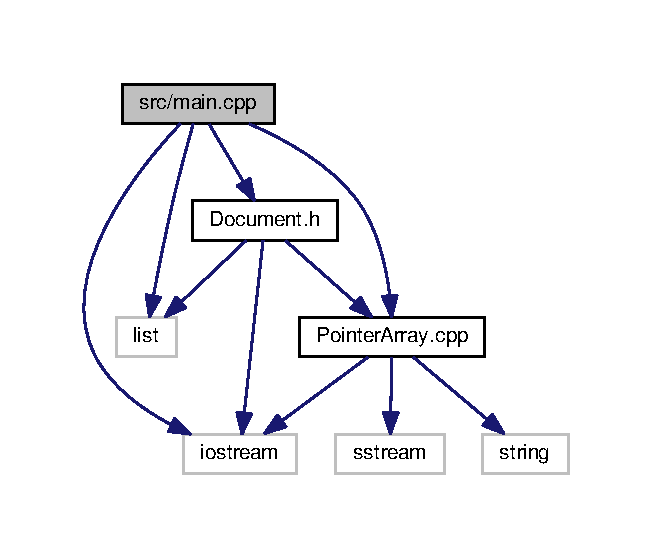
\includegraphics[width=312pt]{main_8cpp__incl}
\end{center}
\end{figure}
\subsection*{Functions}
\begin{DoxyCompactItemize}
\item 
\hypertarget{main_8cpp_aa645d2537e6a806927c27a664653c0f3}{void {\bfseries log\-Test} (std\-::string msg)}\label{main_8cpp_aa645d2537e6a806927c27a664653c0f3}

\item 
int \hyperlink{main_8cpp_ae66f6b31b5ad750f1fe042a706a4e3d4}{main} ()
\begin{DoxyCompactList}\small\item\em the main function to check project consistency by console logging \end{DoxyCompactList}\end{DoxyCompactItemize}


\subsection{Detailed Description}
implements a main function to check the behavior of the \#plist template class and \hyperlink{namespacedocs}{docs} hierarchy. \begin{DoxyAuthor}{Author}
Buoncompagni Luca 
\end{DoxyAuthor}
\begin{DoxyDate}{Date}
Sep 17, 2016
\end{DoxyDate}
\begin{DoxySeeAlso}{See Also}
String\-Pointer\-Array 

plist 

Document 

Spread\-Sheet 

Web\-Page 

\hyperlink{namespacedocs}{docs} 
\end{DoxySeeAlso}


\subsection{Function Documentation}
\hypertarget{main_8cpp_ae66f6b31b5ad750f1fe042a706a4e3d4}{\index{main.\-cpp@{main.\-cpp}!main@{main}}
\index{main@{main}!main.cpp@{main.\-cpp}}
\subsubsection[{main}]{\setlength{\rightskip}{0pt plus 5cm}int main (
\begin{DoxyParamCaption}
{}
\end{DoxyParamCaption}
)}}\label{main_8cpp_ae66f6b31b5ad750f1fe042a706a4e3d4}


the main function to check project consistency by console logging 

check the behavior of the template implementation (\hyperlink{namespaceparray}{parray}) trhough the \#plist\-::\-String\-Pointer\-Array\-::tester() function 

Here is the call graph for this function\-:\nopagebreak
\begin{figure}[H]
\begin{center}
\leavevmode
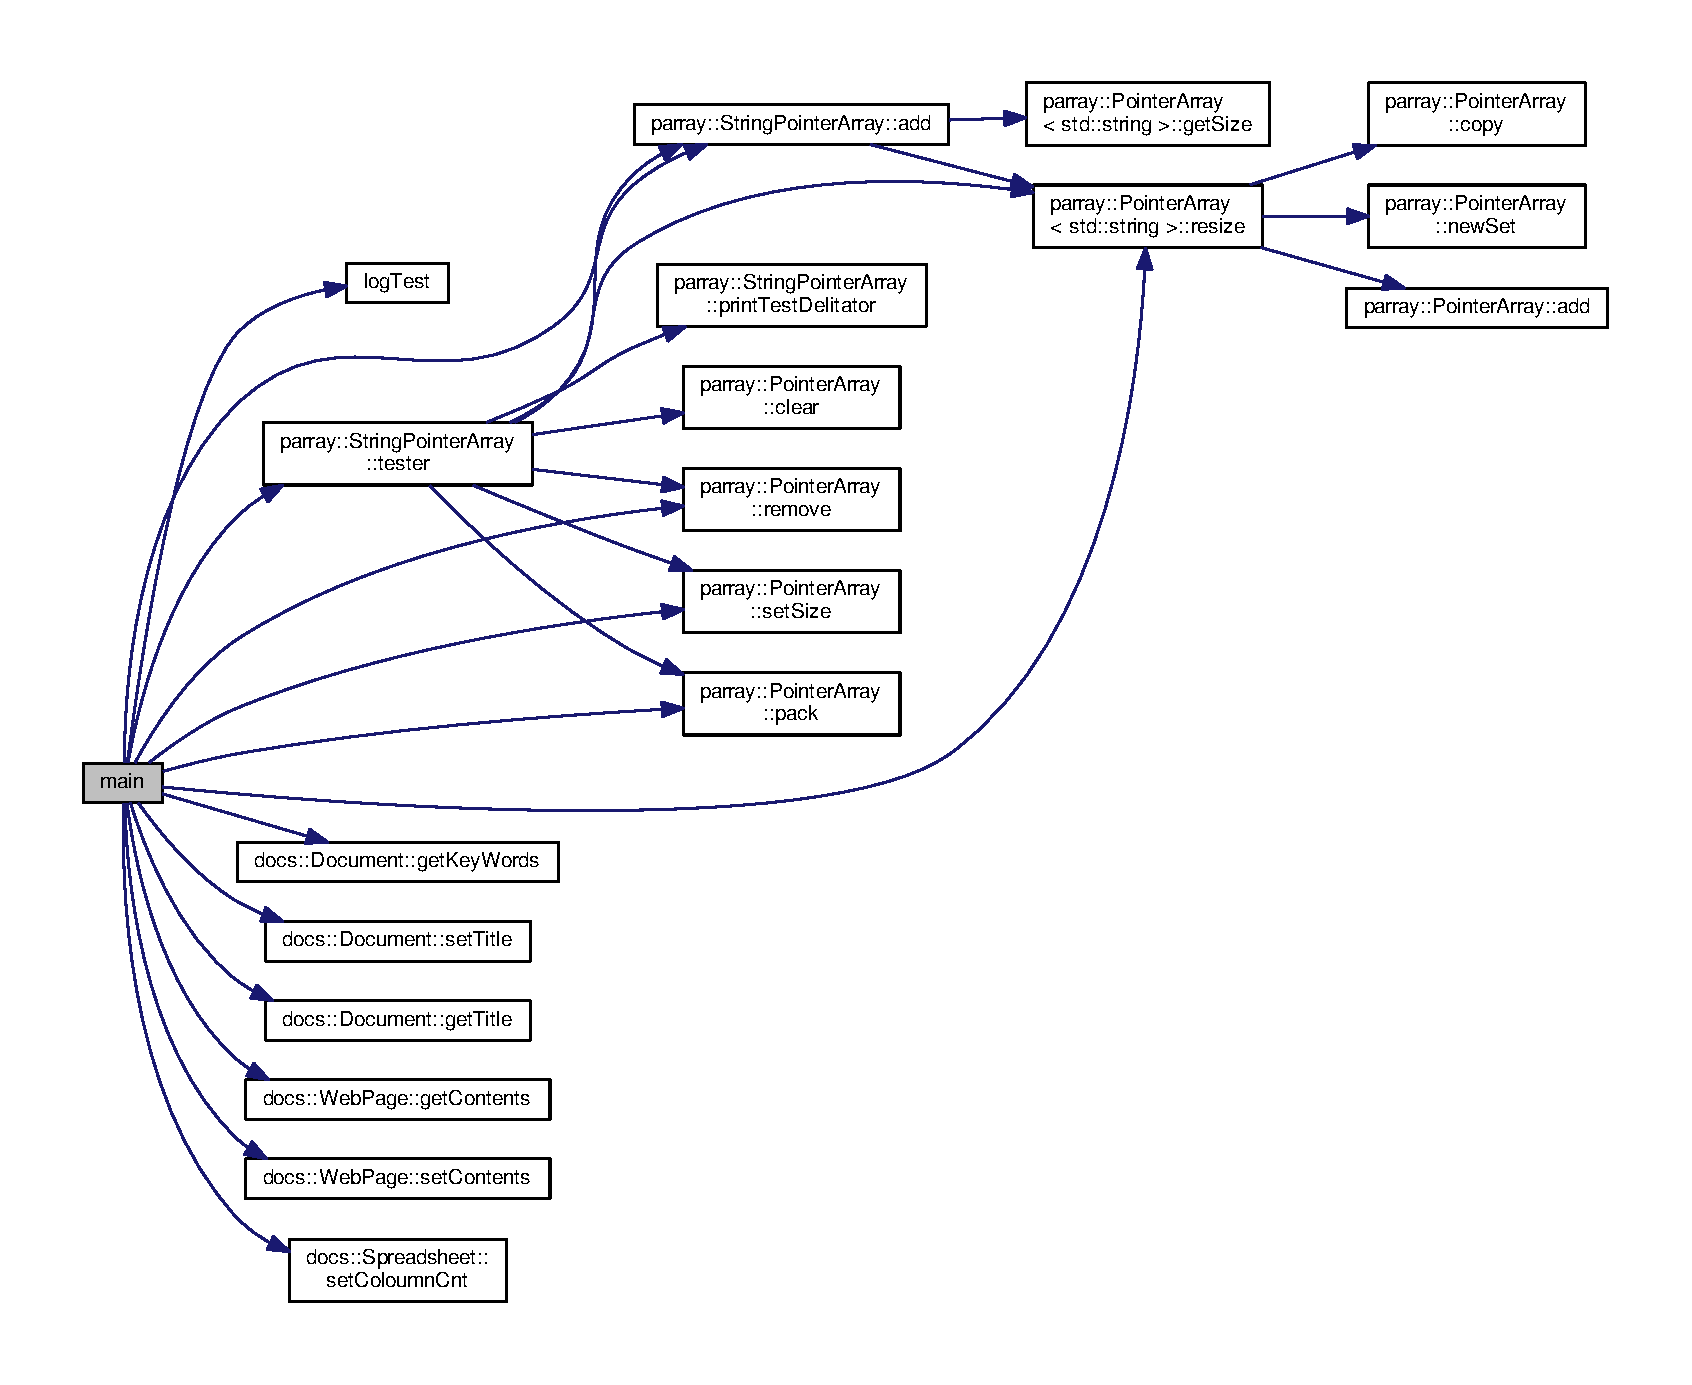
\includegraphics[width=350pt]{main_8cpp_ae66f6b31b5ad750f1fe042a706a4e3d4_cgraph}
\end{center}
\end{figure}



\hypertarget{PointerArray_8cpp}{\section{src/\-Pointer\-Array.cpp File Reference}
\label{PointerArray_8cpp}\index{src/\-Pointer\-Array.\-cpp@{src/\-Pointer\-Array.\-cpp}}
}


The complete \hyperlink{namespaceparray}{parray} (parray\-::\-Pointer\-Array$<$\-T$>$) and \hyperlink{namespacepatch}{patch} names paces definition.  


{\ttfamily \#include $<$iostream$>$}\\*
{\ttfamily \#include $<$sstream$>$}\\*
{\ttfamily \#include $<$string$>$}\\*
Include dependency graph for Pointer\-Array.\-cpp\-:\nopagebreak
\begin{figure}[H]
\begin{center}
\leavevmode
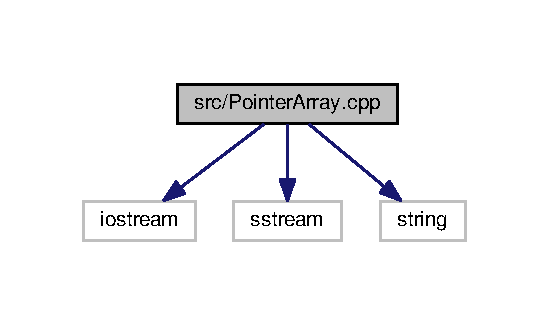
\includegraphics[width=263pt]{PointerArray_8cpp__incl}
\end{center}
\end{figure}
This graph shows which files directly or indirectly include this file\-:\nopagebreak
\begin{figure}[H]
\begin{center}
\leavevmode
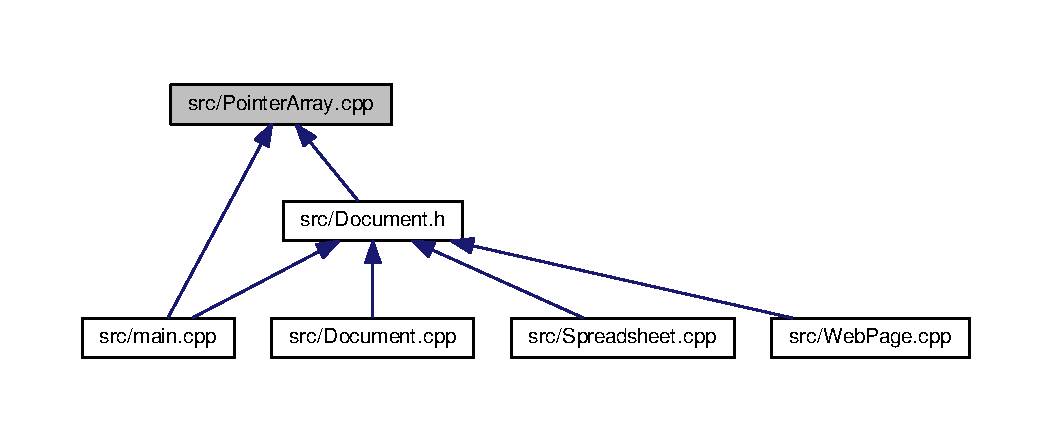
\includegraphics[width=350pt]{PointerArray_8cpp__dep__incl}
\end{center}
\end{figure}
\subsection*{Classes}
\begin{DoxyCompactItemize}
\item 
class \hyperlink{classparray_1_1PointerArray}{parray\-::\-Pointer\-Array$<$ T $>$}
\begin{DoxyCompactList}\small\item\em This class describes a manager of a dynamic array of generic type T$\ast$. \end{DoxyCompactList}\item 
class \hyperlink{classparray_1_1StringPointerArray}{parray\-::\-String\-Pointer\-Array}
\begin{DoxyCompactList}\small\item\em It implements a \hyperlink{classparray_1_1PointerArray_ab506b284822d1e013813579e06893797}{Pointer\-Array} with a string parameter (T). \end{DoxyCompactList}\end{DoxyCompactItemize}
\subsection*{Namespaces}
\begin{DoxyCompactItemize}
\item 
\hyperlink{namespacepatch}{patch}
\begin{DoxyCompactList}\small\item\em to emulate C++11 and get to\-\_\-string translator \end{DoxyCompactList}\item 
\hyperlink{namespaceparray}{parray}
\begin{DoxyCompactList}\small\item\em it specify the dynamic array manager for a generic data T and a std\-::string specialisation. \end{DoxyCompactList}\end{DoxyCompactItemize}
\subsection*{Functions}
\begin{DoxyCompactItemize}
\item 
\hypertarget{namespacepatch_a54d2400c78aef13e3748a87cd7c86ede}{{\footnotesize template$<$typename T $>$ }\\std\-::string \hyperlink{namespacepatch_a54d2400c78aef13e3748a87cd7c86ede}{patch\-::to\-\_\-string} (const T \&n)}\label{namespacepatch_a54d2400c78aef13e3748a87cd7c86ede}

\begin{DoxyCompactList}\small\item\em returns the description of the parameter by using $<$$<$ operator on a fresh std\-::ostringstream \end{DoxyCompactList}\end{DoxyCompactItemize}
\subsection*{Variables}
\begin{DoxyCompactItemize}
\item 
\hypertarget{namespaceparray_af364378bce8a0cb4cd0fc4a191684794}{const std\-::string \hyperlink{namespaceparray_af364378bce8a0cb4cd0fc4a191684794}{parray\-::\-L\-O\-G\-\_\-\-H\-E\-A\-D\-E\-R} = \char`\"{} Pointer\-Array\-: \char`\"{}}\label{namespaceparray_af364378bce8a0cb4cd0fc4a191684794}

\begin{DoxyCompactList}\small\item\em the debugging string to be appended on log head by this list manager \end{DoxyCompactList}\item 
\hypertarget{namespaceparray_ab57bc1fd35280f9304abbf9755598710}{const std\-::string \hyperlink{namespaceparray_ab57bc1fd35280f9304abbf9755598710}{parray\-::\-L\-O\-G\-\_\-\-H\-E\-A\-D\-E\-R\-\_\-\-T\-E\-S\-T} = \char`\"{}\textbackslash{}t\mbox{[}T\-E\-S\-T\mbox{]} \char`\"{} + L\-O\-G\-\_\-\-H\-E\-A\-D\-E\-R}\label{namespaceparray_ab57bc1fd35280f9304abbf9755598710}

\begin{DoxyCompactList}\small\item\em the debugging string to be appended on log head by the \hyperlink{classparray_1_1StringPointerArray_abfac13570bec8c88311714d19ddea59b}{String\-Pointer\-Array\-::tester()} for Test logs \end{DoxyCompactList}\item 
\hypertarget{namespaceparray_a401700c1e4afddc55b1d33cbbc9327db}{const std\-::string \hyperlink{namespaceparray_a401700c1e4afddc55b1d33cbbc9327db}{parray\-::\-L\-O\-G\-\_\-\-H\-E\-A\-D\-E\-R\-\_\-\-W\-A\-R\-N\-I\-N\-G} = \char`\"{}\mbox{[}W\-A\-R\-N\-I\-N\-G\mbox{]} \char`\"{} + L\-O\-G\-\_\-\-H\-E\-A\-D\-E\-R}\label{namespaceparray_a401700c1e4afddc55b1d33cbbc9327db}

\begin{DoxyCompactList}\small\item\em the debugging string to be appended on log head by the \hyperlink{classparray_1_1StringPointerArray_abfac13570bec8c88311714d19ddea59b}{String\-Pointer\-Array\-::tester()} for Warning logs \end{DoxyCompactList}\item 
\hypertarget{namespaceparray_ae12e5e44ecdf5808872ebdc05476e93f}{const std\-::string \hyperlink{namespaceparray_ae12e5e44ecdf5808872ebdc05476e93f}{parray\-::\-L\-O\-G\-\_\-\-H\-E\-A\-D\-E\-R\-\_\-\-I\-N\-F\-O} = \char`\"{}\mbox{[}I\-N\-F\-O\mbox{]} \char`\"{} + L\-O\-G\-\_\-\-H\-E\-A\-D\-E\-R}\label{namespaceparray_ae12e5e44ecdf5808872ebdc05476e93f}

\begin{DoxyCompactList}\small\item\em the debugging string to be appended on log head by the \hyperlink{classparray_1_1StringPointerArray_abfac13570bec8c88311714d19ddea59b}{String\-Pointer\-Array\-::tester()} for Info logs \end{DoxyCompactList}\item 
\hypertarget{namespaceparray_a6cd699f2dd9c98d7f9ac98fb178a8a4f}{const std\-::string \hyperlink{namespaceparray_a6cd699f2dd9c98d7f9ac98fb178a8a4f}{parray\-::\-L\-O\-G\-\_\-\-H\-E\-A\-D\-E\-R\-\_\-\-E\-R\-R\-O\-R} = \char`\"{}\mbox{[}E\-R\-R\-O\-R\mbox{]} \char`\"{} + L\-O\-G\-\_\-\-H\-E\-A\-D\-E\-R}\label{namespaceparray_a6cd699f2dd9c98d7f9ac98fb178a8a4f}

\begin{DoxyCompactList}\small\item\em the debugging string to be appended on log head by the \hyperlink{classparray_1_1StringPointerArray_abfac13570bec8c88311714d19ddea59b}{String\-Pointer\-Array\-::tester()} for Error logs \end{DoxyCompactList}\end{DoxyCompactItemize}


\subsection{Detailed Description}
The complete \hyperlink{namespaceparray}{parray} (parray\-::\-Pointer\-Array$<$\-T$>$) and \hyperlink{namespacepatch}{patch} names paces definition. \begin{DoxyAuthor}{Author}
Buoncompagni Luca 
\end{DoxyAuthor}
\begin{DoxyDate}{Date}
Sep 14, 2016
\end{DoxyDate}
It describes a common templated method to convert an object into a string (\hyperlink{namespacepatch_a54d2400c78aef13e3748a87cd7c86ede}{patch\-::to\-\_\-string()}). Also, it defines a templated manager to a dynamic array (\hyperlink{classparray_1_1PointerArray}{parray\-::\-Pointer\-Array}) as well as a specialisation that deal with arrays of string (\hyperlink{classparray_1_1StringPointerArray}{parray\-::\-String\-Pointer\-Array}). For the last, also a static method for behavior testing is provided (String\-Pointer\-Array\-::tester()). 

Definition in file \hyperlink{PointerArray_8cpp_source}{Pointer\-Array.\-cpp}.


\hypertarget{Spreadsheet_8cpp}{\section{src/\-Spreadsheet.cpp File Reference}
\label{Spreadsheet_8cpp}\index{src/\-Spreadsheet.\-cpp@{src/\-Spreadsheet.\-cpp}}
}


implementation of the Spreadsheet (extending) Document class.  


{\ttfamily \#include \char`\"{}Document.\-h\char`\"{}}\\*
Include dependency graph for Spreadsheet.\-cpp\-:\nopagebreak
\begin{figure}[H]
\begin{center}
\leavevmode
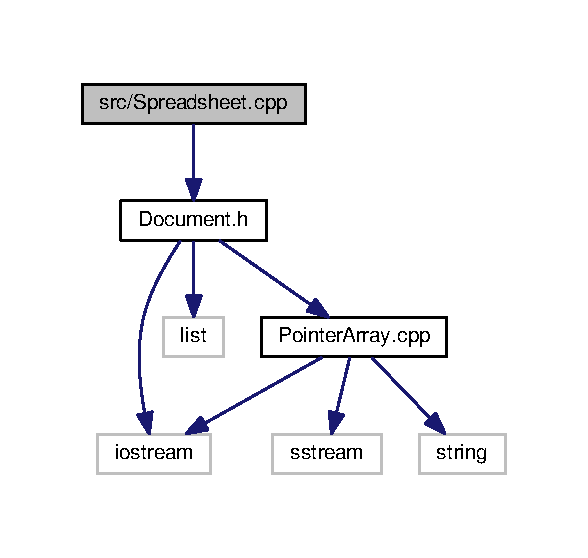
\includegraphics[width=282pt]{Spreadsheet_8cpp__incl}
\end{center}
\end{figure}
\subsection*{Namespaces}
\begin{DoxyCompactItemize}
\item 
\hyperlink{namespacedocs}{docs}
\begin{DoxyCompactList}\small\item\em This namespace is used to collect all the document hierarchy classes and types. \end{DoxyCompactList}\end{DoxyCompactItemize}


\subsection{Detailed Description}
implementation of the Spreadsheet (extending) Document class. \begin{DoxyAuthor}{Author}
Buoncompagni Luca 
\end{DoxyAuthor}
\begin{DoxyDate}{Date}
Sep 14, 2016
\end{DoxyDate}
\begin{DoxySeeAlso}{See Also}
Spreadsheet 

Document 

\hyperlink{namespacedocs}{docs} 
\end{DoxySeeAlso}

\hypertarget{WebPage_8cpp}{\section{src/\-Web\-Page.cpp File Reference}
\label{WebPage_8cpp}\index{src/\-Web\-Page.\-cpp@{src/\-Web\-Page.\-cpp}}
}


implementation of the \hyperlink{classdocs_1_1WebPage}{docs\-::\-Web\-Page} class.  


{\ttfamily \#include \char`\"{}Document.\-h\char`\"{}}\\*
Include dependency graph for Web\-Page.\-cpp\-:\nopagebreak
\begin{figure}[H]
\begin{center}
\leavevmode
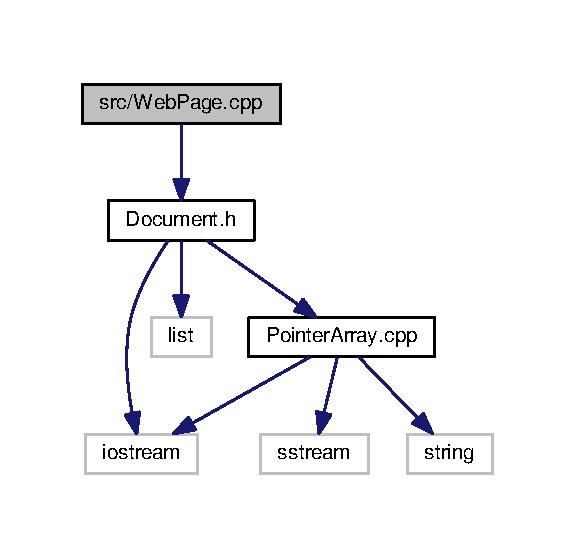
\includegraphics[width=276pt]{WebPage_8cpp__incl}
\end{center}
\end{figure}
\subsection*{Namespaces}
\begin{DoxyCompactItemize}
\item 
\hyperlink{namespacedocs}{docs}
\begin{DoxyCompactList}\small\item\em This namespace is used to collect all the document hierarchy classes and types. \end{DoxyCompactList}\end{DoxyCompactItemize}


\subsection{Detailed Description}
implementation of the \hyperlink{classdocs_1_1WebPage}{docs\-::\-Web\-Page} class. \begin{DoxyAuthor}{Author}
Buoncompagni Luca 
\end{DoxyAuthor}
\begin{DoxyDate}{Date}
Sep 14, 2016
\end{DoxyDate}
\begin{DoxySeeAlso}{See Also}
Web\-Page 

Document 

\hyperlink{namespacedocs}{docs} 
\end{DoxySeeAlso}

%--- End generated contents ---

% Index
\newpage
\phantomsection
\addcontentsline{toc}{chapter}{Index}
\printindex

\end{document}
